%%
%% This is file `sample-sigplan.tex',
%% generated with the docstrip utility.
%%
%% The original source files were:
%%
%% samples.dtx  (with options: `sigplan')
%% 
%% IMPORTANT NOTICE:
%% 
%% For the copyright see the source file.
%% 

%% Any modified versions of this file must be renamed
%% with new filenames distinct from sample-sigplan.tex.
%% 
%% For distribution of the original source see the terms
%% for copying and modification in the file samples.dtx.
%% 
%% This generated file may be distributed as long as the
%% original source files, as listed above, are part of the
%% same distribution. (The sources need not necessarily be
%% in the same archive or directory.)
%%
%% Commands for TeXCount
%TC:macro \cite [option:text,text]
%TC:macro \citep [option:text,text]
%TC:macro \citet [option:text,text]
%TC:envir table 0 1
%TC:envir table* 0 1
%TC:envir tabular [ignore] word
%TC:envir displaymath 0 word
%TC:envir math 0 word
%TC:envir comment 0 0
%%
%%
%% The first command in your LaTeX source must be the \documentclass command.
\documentclass[sigplan,screen]{acmart}
\usepackage{algorithm} 
\usepackage[noend]{algpseudocode} 
\usepackage[titles]{tocloft}
\usepackage{tikz}
\usepackage{listings}
\usepackage{xspace}
\usepackage{tcolorbox}
\usepackage{multirow}
\usepackage{adjustbox}
\usepackage[inline]{enumitem}
\usepackage{xspace}
\usepackage[listings,skins]{tcolorbox}


\AtBeginDocument{%
  \providecommand\BibTeX{{%
    \normalfont B\kern-0.5em{\scshape i\kern-0.25em b}\kern-0.8em\TeX}}}

%% Rights management information.  This information is sent to you
%% when you complete the rights form.  These commands have SAMPLE
%% values in them; it is your responsibility as an author to replace
%% the commands and values with those provided to you when you
%% complete the rights form.
\setcopyright{acmcopyright}
\copyrightyear{2018}
\acmYear{2018}
\acmDOI{XXXXXXX.XXXXXXX}

%% These commands are for a PROCEEDINGS abstract or paper.
\acmConference[Conference acronym 'XX]{Make sure to enter the correct
  conference title from your rights confirmation emai}{June 03--05,
  2018}{Woodstock, NY}
%
%  Uncomment \acmBooktitle if th title of the proceedings is different
%  from ``Proceedings of ...''!
%
%\acmBooktitle{Woodstock '18: ACM Symposium on Neural Gaze Detection,
%  June 03--05, 2018, Woodstock, NY} 
\acmPrice{15.00}
\acmISBN{978-1-4503-XXXX-X/18/06}


%%
%% Submission ID.
%% Use this when submitting an article to a sponsored event. You'll
%% receive a unique submission ID from the organizers
%% of the event, and this ID should be used as the parameter to this command.
%%\acmSubmissionID{123-A56-BU3}

%%
%% For managing citations, it is recommended to use bibliography
%% files in BibTeX format.
%%
%% You can then either use BibTeX with the ACM-Reference-Format style,
%% or BibLaTeX with the acmnumeric or acmauthoryear sytles, that include
%% support for advanced citation of software artefact from the
%% biblatex-software package, also separately available on CTAN.
%%
%% Look at the sample-*-biblatex.tex files for templates showcasing
%% the biblatex styles.
%%

%%
%% The majority of ACM publications use numbered citations and
%% references.  The command \citestyle{authoryear} switches to the
%% "author year" style.
%%
%% If you are preparing content for an event
%% sponsored by ACM SIGGRAPH, you must use the "author year" style of
%% citations and references.
%% Uncommenting
%% the next command will enable that style.
%%\citestyle{acmauthoryear}


\makeatletter


\newenvironment{btHighlight}[1][]
{\begingroup\tikzset{bt@Highlight@par/.style={#1}}\begin{lrbox}{\@tempboxa}}
{\end{lrbox}\bt@HL@box[bt@Highlight@par]{\@tempboxa}\endgroup}


\definecolor{commentgreen}{RGB}{176, 176, 176}
\definecolor{rowcolor}{cmyk}{0,0.87,0.68,0.32}
\definecolor{rowcolor2}{cmyk}{ 20, 0, 37, 34}

\definecolor{eminence}{RGB}{108,48,130}
\definecolor{weborange}{RGB}{255,165,0}
\definecolor{frenchplum}{RGB}{129,20,82}
\definecolor{darkgreen}{RGB}{10, 92, 10}

\definecolor{celadon}{rgb}{0.67, 0.88, 0.69}
%\renewcommand{\blue}{}

\newcommand\btHL[1][]{%
  \begin{btHighlight}[#1]\bgroup\aftergroup\bt@HL@endenv%
}
\def\bt@HL@endenv{%
  \end{btHighlight}%   
  \egroup
}
\newcommand{\bt@HL@box}[2][]{%
  \tikz[#1]{%
    \pgfpathrectangle{\pgfpoint{1pt}{0pt}}{\pgfpoint{\wd #2}{\ht #2}}%
    \pgfusepath{use as bounding box}%
    \node[anchor=base west, fill=orange!30,outer sep=0pt,inner xsep=1pt, inner ysep=0pt, rounded corners=3pt, minimum height=\ht\strutbox+1pt,#1]{\raisebox{1pt}{\strut}\strut\usebox{#2}};
  }%
}
\makeatother
\newcommand*\badge[1]{ \colorbox{red}{\color{white}#1}}
\newcommand{\tool}{Wasm-mutate\xspace}
\newcommand{\wasm}{Wasm\xspace}
\newcommand{\Wasm}{WebAssembly\xspace}
\newcommand{\etal}{et.al.\xspace}
\newcommand{\ie}{i.e.,\xspace}

\newtheorem{definition}{Definition}
\providecommand*{\definitionautorefname}{Definition}
\newtheorem{metric}{Metric}
\providecommand*{\metricautorefname}{Metric}

\newlistof{todo}{td}{List of TODOs}

\newcommand{\revision}[1]{{\textcolor{red}{#1}}}
\newcommand{\repourl}{\url{https://github.com/Jacarte/wasm_evasion}}

\newcommand{\todo}[1]{%
\refstepcounter{todo}
\noindent\textbf{\badge{TODO}} {\color{red}#1}
\addcontentsline{td}{todo}
{\color{red}\thesection.\thetodo\xspace #1}}


% Define the WAT language
\lstdefinelanguage{WAT}{
    otherkeywords={},
    morekeywords=[1]{i32,f32,i64,f64,funcref, nop},
    morekeywords=[2]{0},
    morekeywords=[3]{add,or,const,mul,eqz,shl,get,rem_s,rem_u,ne,tee,sub,set,store},
    morekeywords=[4]{},
    morekeywords=[5]{global, get_global, mut, set_global, export, import,loop, memory, data, get_local,if,element, block,module, function, set_local,call,br_if,end,br, else, all,call_indirect,local,global,module, func, param, result, type, table, memory, elem},
    morekeywords=[6]{=,;},
    morekeywords=[7]{(,),[,],.},
    sensitive=false,
    morecomment=[l]{;},
    morecomment=[s]{;}{;},
    morestring=[b]",
    keywordstyle=[1]\color{eminence}\bfseries,
    keywordstyle=[3]\color{frenchplum},
    keywordstyle=[5]\color{darkgreen}\bfseries,
    commentstyle=\color{commentgreen}
}
\lstdefinestyle{nccode}{
        numbers=none,
        firstnumber=2,
        stepnumber=1,
        numbersep=10pt,
        tabsize=4, 
        showspaces=false,
        breaklines=true, 
        showstringspaces=false,
    %moredelim=**[is][\btHL]{`}{`},
    moredelim=**[is][{\btHL[fill=weborange!40]}]{`}{`},
    moredelim=**[is][{\btHL[fill=celadon!40]}]{!}{!}
}

\lstdefinestyle{WATStyle}{
  numbers=left,
  stepnumber=1,
  numbersep=10pt,
  tabsize=4,
  showspaces=false,
  showstringspaces=true,
}



\newcommand\tikzmarkWS[4]{%
\tikz[remember picture, overlay]{%
        \pgfusepath{use as bounding box}%
        \node[right=#3 mm, fill=white!0] at (1 mm,2 mm) (#1) {#2};
      %\node[right=#3 mm, align=center, shape=circle,text=black,draw=black, fill=white,inner sep=0.5pt] (#1) {#2};
  }
 }

  
 \newcommand\tikzmarkPROBE[4]{%
\tikz[remember picture, overlay]{%
        \pgfusepath{use as bounding box}%
        \node[right=#3 mm,text width=2mm,align =center,outer sep=0pt,inner xsep=1pt, inner ysep=0pt, rounded corners=3pt,anchor=north, minimum height=#4 mm, text depth = #4 mm] at (1 mm,2 mm) (#1) {};
      %\node[right=#3 mm, align=center, shape=circle,text=black,draw=black, fill=white,inner sep=0.5pt] (#1) {#2};
  }
 }

 % Replacement of the texttt command
 \lstdefinelanguage{ttt}{
    otherkeywords={},
    morekeywords=[1]{i32,f32,i64,f64,funcref,x,nop},
    morekeywords=[2]{0},
    morekeywords=[3]{container, add,const,mul,shl,get,rem_s,eqz,rem_u,ne,tee,sub,set,store,or},
    morekeywords=[4]{},
    morekeywords=[5]{global, get_global, mut, set_global, export, import,loop, memory, data, get_local,if, block,module, set_local,call,br_if,end,br, else, ret,all,call_indirect,local,global,module, func, param, result, type, table, (, ), memory, elem},
    morekeywords=[6]{=,;},
    morekeywords=[7]{[,],.},
    morekeywords=[8]{LHS, RHS, Cond},
    sensitive=false,
    morecomment=[l]{;},
    morecomment=[s]{;}{;},
    morestring=[b]",
    keywordstyle=[1]\color{eminence}\bfseries,
    keywordstyle=[3]\color{frenchplum},
    keywordstyle=[5]\color{darkgreen}\bfseries,
    keywordstyle=[7]\color{darkgreen}\bfseries,
    keywordstyle=[8]\color{frenchplum}\bfseries,
    keywordstyle=[2]\color{darkgreen}\bfseries,
    commentstyle=\color{commentgreen}
}
 \lstset{
    frameround=fttt,
    language=ttt,
    numbers=left,
    breaklines=true,
    basicstyle=\small\ttfamily
    }
 \renewcommand{\texttt}[1]{\lstinline{#1}}

 \lstdefinelanguage{TRACE}{
    otherkeywords={},
    morekeywords=[1]{dword, qword,ptr},
    morekeywords=[2]{0},
    morekeywords=[3]{mov, value, size, Writ, Read, I},
    morekeywords=[4]{rdx, ecx, r14},
    morekeywords=[5]{global, get_global, mut, set_global, export, import,loop, memory, data, get_local,if,element, block,module, function, set_local,call,br_if,end,br, else, all,call_indirect,local,global,module, func, param, result, type, table, memory, elem},
    morekeywords=[6]{=,;},
    morekeywords=[7]{(,),[,],.},
    sensitive=false,
    morecomment=[l]{;},
    morecomment=[s]{;}{;},
    morestring=[b]",
    keywordstyle=[1]\color{eminence}\bfseries,
    keywordstyle=[3]\color{frenchplum},
    keywordstyle=[5]\color{darkgreen}\bfseries,
    commentstyle=\color{commentgreen}
}

%%
%% end of the preamble, start of the body of the document source.
\begin{document}

%%
%% The "title" command has an optional parameter,
%% allowing the author to define a "short title" to be used in page headers.
\title{WebAssembly Binary Diversification with Guarantees}


%%
%% By default, the full list of authors will be used in the page
%% headers. Often, this list is too long, and will overlap
%% other information printed in the page headers. This command allows
%% the author to define a more concise list
%% of authors' names for this purpose.

%%
%% The abstract is a short summary of the work to be presented in the
%% article.
\begin{abstract}
  
\end{abstract}

%%
%% The code below is generated by the tool at http://dl.acm.org/ccs.cfm.
%% Please copy and paste the code instead of the example below.
%%
\begin{CCSXML}
<ccs2012>
 <concept>
  <concept_id>10010520.10010553.10010562</concept_id>
  <concept_desc>Computer systems organization~Embedded systems</concept_desc>
  <concept_significance>500</concept_significance>
 </concept>
 <concept>
  <concept_id>10010520.10010575.10010755</concept_id>
  <concept_desc>Computer systems organization~Redundancy</concept_desc>
  <concept_significance>300</concept_significance>
 </concept>
 <concept>
  <concept_id>10010520.10010553.10010554</concept_id>
  <concept_desc>Computer systems organization~Robotics</concept_desc>
  <concept_significance>100</concept_significance>
 </concept>
 <concept>
  <concept_id>10003033.10003083.10003095</concept_id>
  <concept_desc>Networks~Network reliability</concept_desc>
  <concept_significance>100</concept_significance>
 </concept>
</ccs2012>
\end{CCSXML}

\ccsdesc[500]{Computer systems organization~Embedded systems}
\ccsdesc[300]{Computer systems organization~Redundancy}
\ccsdesc{Computer systems organization~Robotics}
\ccsdesc[100]{Networks~Network reliability}

%%
%% Keywords. The author(s) should pick words that accurately describe
%% the work being presented. Separate the keywords with commas.
\keywords{datasets, neural networks, gaze detection, text tagging}

%% A "teaser" image appears between the author and affiliation
%% information and the body of the document, and typically spans the
%% page.

%%
%% This command processes the author and affiliation and title
%% information and builds the first part of the formatted document.
\maketitle

%%
%% The next two lines define the bibliography style to be used, and
%% the bibliography file.

\section{Introduction}

- For the security motivation, The Security Risk of Lacking Compiler Protection in WebAssembly \cite{stievenart2021security}

motivate with th CVE in Fastly case, semantically aware transformations are good in some specific cases. 

- Wasm-mutate is a completement for wasm-smith and they must be used together. For example, wasm-mutate is not able to create loops from scratch, while wasm-smith can. Since the need is speed, each implementation is done as fast as possible. This relies on the backend implementation of code generation to optimize and generate performance code.

- Ephasize that Wasm 2 Wasm is better.  The limitations for CROW and MEWE. They are based on LLVM. They use a theorem solver, which is extremely slow. The same theorem solver could be used to curate the rewriting rules. LLVM onlu accounts for 70\% of the Wasm binaries in the wild. Now we have Javy and other compilers support Wasm. Wasm 2 wasm solution is impeorative.

- Cache tming: \cite{Genkin2018DrivebyKC}
The original POC programs are wholly vulnerable to attacks. 
This risk dramatically escalates when the binary is replicated and potentially executed across a multitude of machines worldwide, such as in a Function-as-a-Service (FaaS) platform like Fastly \cite{MEWE}.
In concrete, distributing the unmodified binary to 100 machines would, essentially, creates 100 homogeneously vulnerable machines.
However, let us illustrate the case with a different approach: each time the binary is replicated onto a different machine, we distribute a unique variant instead of the original binary. 
If we disseminate a unique variant, with X stacked transformations, to each machine, every system would run a distinct \wasm binary. 
Based on our findings, even when some binaries are still vulnerable, we can confidently say that if 100 variants of a vulnerable program, each furnished with X stacked transformations, are distributed, the impact of any potential attack is considerably mitigated.
While it's true that some variants may retain their original vulnerabilities, not all of them do. 
This significantly enhances overall security. 
Further reinforcing this point, let's consider the case of btb\_leakage. 
In this scenario, a suite of 100 variants, each featuring at least 200 stacked transformations, ensures full protection against potential threats, effectively securing the entire infrastructure.
Moreover, considering the results for the ret2spec attack, this property holds for the whole population of generated variants, despite the number of stacked transformations.
Therefore, \tool as a software diversification tool, is a peemptive solution to potential attacks.


- Second, wasm-mutate takes from CROW its rewriting rules.

To sum up, the contributions of this work are:

\begin{itemize}
    \item \tool, a tool tailored for WebAssembly to WebAssembly software diversification.
    \item Empirical evidence on static and dynamic differences provided by the variants created by \tool.
    \item Empirical evidence on how \tool can protect cache timing side-channel attacks.
    \item Empirical evidence on how \tool can be used to conduct differential testing.
    
\end{itemize}

\section{Background}

In this section, we define and formulate the foundation of this work: WebAssembly, its runtime structure, semantic equivalence modulo input, rewriting rules and e-graphs.
Along with the paper, we use the terms, metrics and concepts defined here.

\subsection{WebAssembly}

WebAssembly (Wasm) is a binary instruction set initially  meant for the web, and now also used in the backend. 
It was adopted as a standardized language by the W3C in 2017, building upon the work of Haas et al. \cite{haas2017bringing}. One of Wasm's primary advantages is that it defines its own Instruction Set Architecture (ISA), which is both platform-independent. As a result, a Wasm binary can execute on virtually any platform, including web browsers and server-side environments. 
WebAssembly programs are compiled ahead-of-time from source languages such as C/C++, Rust, and Go, utilizing compilation pipelines like LLVM. 



\lstdefinestyle{watcode}{
  numbers=none,
  stepnumber=1,
  numbersep=10pt,
  tabsize=4,
  showspaces=false,
  breaklines=true, 
  showstringspaces=false,
  moredelim=**[is][{\btHL[fill=black!10]}]{`}{`},
  moredelim=**[is][{\btHL[fill=celadon!40]}]{!}{!}
}
{
%\captionsetup{width=0.9\linewidth}
\lstset{
  language=WAT,
  style=watcode,
  breaklines=true, 
  basicstyle=\footnotesize\ttfamily,
  %numberstyle=\footnotesize,
  numbersep=2.5pt,
  %firstnumber=1,
  escapeinside={``},
  %numbers=left,
  %postbreak=\mbox{\textcolor{red}{$\hookrightarrow$}\space},
  }
    \begin{lstlisting}[label=example:wasmprogram,caption={Simplified WebAssembly code for the program of \autoref{example:cprogram}.}, captionpos=b]{Name}
(module
  (@custom "producer" "llvm.." )
  (import "env" "println" (func $println (param i32)))
  (memory 1)
  (export "memory" (memory 0))
  (func $main
    (local $sum i32)
    (local $i i32)
    (local $arr_offset i32)
    ; Initialize sum to 0 ;
    i32.const 0
    local.set $sum
    ; Initialize arr_offset to point to start of the array in memory ;
    i32.const 0
    local.set $arr_offset
    ; Initialize the array in memory;
    i32.const 0
    i32.const 1
    i32.store
    ...
    i32.store
    ...
    loop
      local.get $i
      i32.const 5
      i32.lt_s
      if
        ; Load array[i] and add to sum ;
        local.get $arr_offset
        local.get $i
        ...
        ; Increment i ;
        local.get $i
        i32.const 1
        i32.add
        local.set $i
        br 0
      else
        ; End loop ;
        i32.const 0
      end
    end
    
    ; Call external function to print sum ;
    local.get $sum
    call $println
  )
  ; Start the main function ;
  (start $main)
  )
\end{lstlisting}
}


% We do not enumerate the types, lets try to be as much agnostic to the version of Wasm as possible
WebAssembly programs operate on a virtual stack that allows primitive data types.
% These same data types are used to annotate instructions in the WebAssembly code.
Additionally, a WebAssembly program might include several custom sections.
For example, binary producers such as compilers use custom sections to store metadata, such as the name of the compiler that generates the Wasm code.
A WebAssembly program also declares memory sections and globals, which are used to store, manipulate and share data during program execution, e.g. to share data with the host engine of the WebAssembly binary.

WebAssembly is designed with isolation as a primary consideration. For instance, a WebAssembly binary cannot access the memory of other binaries or cannnot interact directly with browser's APIs, such as the DOM or the network. Instead, communication with these features is constrained to functions imported from the host engine, ensuring a secure and safe Wasm environment.
Moreover, control flow in WebAssembly is managed through explicit labels and well-defined blocks, which means that jumps in the program can only occur inside blocks, unlike regular assembly code \cite{10.1145/3062341.3062363}. 
\todo{Change the example to Rust}
In \autoref{example:cprogram}, we provide an example of a C program that contains a function declaration, a loop, a loop conditional, and a memory access. When the C code is compiled to WebAssembly, it produces the code shown in \autoref{example:wasmprogram}. The stack operations are folded with parentheses.
The module in the example contains the components described previously.

% Now we talk a bit about what is the state of a Wasm program.
%\todo{The following text should be revised. }

The WebAssembly runtime structure is described in the WebAssembly specification and it includes 10 key elements: the Store, Stack, Locals, Module Instances, Function Instances, Table Instances, Memory Instances, Global Instances, Export Instances, and Import Instances. These components interact during the execution of a WebAssembly program, collectively defining the state of a program during its runtime.

Two of these elements, the Stack and Memory instances, are particularly significant in maintaining the state of a WebAssembly program during its execution. The Stack holds both values and control frames, with control frames handling block instructions, loops, and function calls. Meanwhile, Memory Instances represent the linear memory of a WebAssembly program, consisting of a contiguous array of bytes.
In this paper, we highlight the aforementioned two components to define, compare and validate the state of two Wasm programs during their execution. 

\subsection{Semantic Equivalence}

Semantic equivalence refers to the notion that two programs or functions are considered equivalent if, for a given specified input domain, they produce the same output values or have the same observable behavior \cite{Semantic equivalence}. 
In other words, the semantics of the two programs are equivalent when the input-output relationship (w/ possibly some abstraction), even if the internal implementation details or the structure of the programs differ.


Let us illustrate this with an example.
Assume two programs $P$ and $P'$ (\autoref{example:state1} and \autoref{example:state2} respectively) where $P'$ is the result of modifying a code in the first instruction of its unique function.
The program $P'$ has two extra instructions right before returning from the function.
The remaining components of the original binary are not modified.



\lstdefinestyle{watcode}{
  numbers=none,
  stepnumber=1,
  numbersep=10pt,
  tabsize=4,
  showspaces=false,
  breaklines=true, 
  showstringspaces=false,
    moredelim=**[is][{\btHL[fill=weborange!40]}]{`}{`},
    moredelim=**[is][{\btHL[fill=celadon!40]}]{!}{!}
}
   \begin{minipage}[t]{0.45\linewidth}
    \lstset{
        language=WAT,
                        style=watcode,
        basicstyle=\footnotesize\ttfamily,
                        columns=fullflexible,
                        breaklines=true}
        
        \begin{lstlisting}[label=example:state1,caption={Program P.},frame=b, captionpos=b]{state1}
func (;0;) (type 0) (param i32 f32) (result i64)
    i64.const 1
        \end{lstlisting}
\end{minipage}\hfill
\begin{minipage}[t]{0.45\linewidth}
    \lstset{
        language=WAT,
                        style=watcode,
        basicstyle=\footnotesize\ttfamily,
                        columns=fullflexible,
                        breaklines=true}
        
        \begin{lstlisting}[label=example:state2,caption={Program $P'$, transformation of program $P$.},frame=b, captionpos=b]{state2}
func (;0;) (type 0) (param i32 f32) (result i64)
    i64.const 1
    !i32.const 42!
    !i32.drop!
        \end{lstlisting}
\end{minipage}


The state of the program $P$ when entering the function is its stack $[S]$, 
the program $P'$ has the same state before executing the function.
The input values of the function for both programs are $L$, their outputs are the top of the stack at the end of the execution.


Program $P$ has the state $[[S:i32.const\ 1]]$ just before returning from the function execution.
When we trace the states of the program $P'$, we can construct the following sequence of states:
\begin{enumerate}
    \item $[[S: i32.const\ 1]]$ the integer constant 1 is now on the top of the stack.
    \item $[[S: i32.const\ 1, i32.const\ 42]]$ the integer constant 32 is  the top of the stack.
    \item $[[S: i32.const\ 1]]$ the top of the stack is dropped. The function execution stops.
\end{enumerate}
Notice that, the stack state of program $P'$ is the same as program $P$.
Thus, we can say that these two programs are semantically equivalent.
Even though the programs share semantic equivalence, they display differences during execution. 
Specifically, $P'$ stresses more on the stack by adding and subsequently dropping more values.
These subtle yet significant differences form the crux of the diversification approaches discussed in this study.






\subsection{Rewriting rule}
\label{rewriting}

Our definition of a rewriting rule draws from the one proposed by Sasnauskas et al. \cite{2017arXiv171104422S}, and integrates a predicate to specify the replacement condition.
Concretely, a rewriting rule is defined as a tuple, denoted as \texttt{(LHS, RHS, Cond)}. Here, \texttt{LHS} refers to the code segment slated for replacement, \texttt{RHS} is the proposed replacement, and \texttt{Cond} stipulates the conditions under which the replacement is acceptable.
Importantly, \texttt{LHS} and \texttt{RHS} are meant to be semantically equivalent, per the definition of previous section.


For example, the rewriting rule \texttt{(x,\ x\ i32.or\ x, \{\})} implies that the \texttt{LHS} 'x' is to be replaced by an idempotent bitwise \texttt{i32.or} operation with itself, absent any specific conditions.
Notice that, for this specific rule, the commutative property shared by \texttt{LHS} and \texttt{RHS}, symbolized as \texttt{(LHS, RHS) = (RHS, LHS)}.
Besides, the \texttt{Cond} element could be an arbitrary criterion. 
For instance, the condition for applying the aforementioned rewriting rule could be to ensure that the newly created binary file does not exceed a threshold binary size.

Based on our understanding, our research is the first to apply the concept of rewriting rules to WebAssembly.
This will expand the potential use cases of wasm-mutate. 
Beyond its role as a diversification tool, it can also be used as a standard tool for conducting program transformations in WebAssembly.


\section {Design of Wasm-Mutate}

% Here is the state of wasm-mutate \url{https://github.com/bytecodealliance/wasm-tools/issues/415}.

In this section we present \tool, a novel technique to diversify
WebAssembly binaries and produce semantically equivalent variants.

\begin{figure*}[h!]
    \centering
    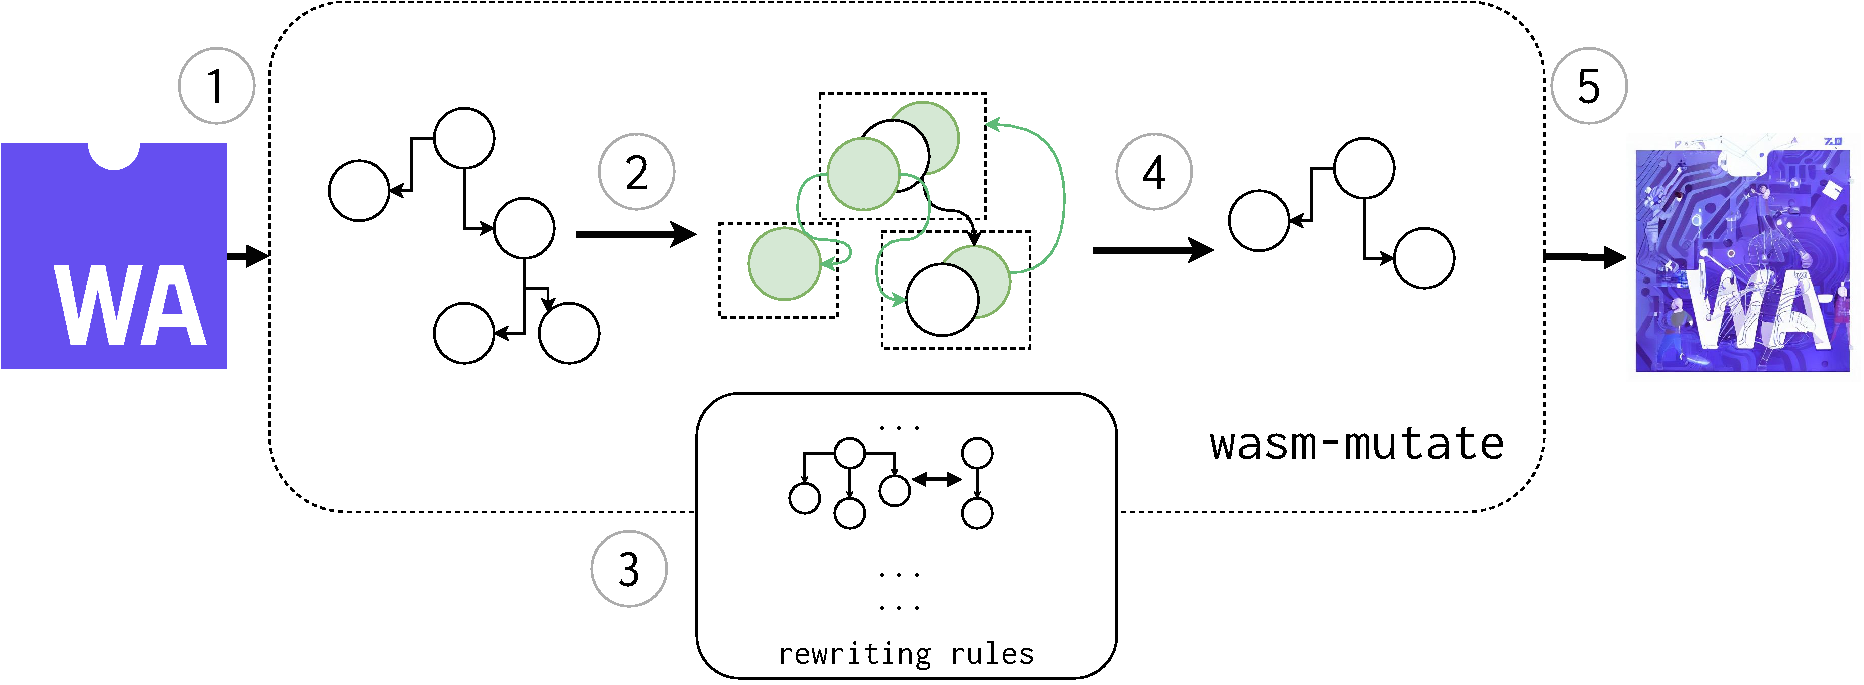
\includegraphics[width=0.8\linewidth]{figures/wasm-mutate-general.pdf}
    \caption{ \tool workflow and high level architecture.}
  \label{fig:wasm-mutate}
\end{figure*}

\subsection{Overview}
The primary objective of \tool is to perform WebAssembly to WebAssembly diversification, i.e., generate semantically equivalent variants from a given WebAssembly binary input. 
\tool's central approach involves synthesizing these variants by substituting parts of the original binary using rewrite rules. 
It leverages a comprehensive set of rewrite rules, boosted by a proposed random traversals of e-graph structures (refer to \autoref{alg}).


In \autoref{fig:wasm-mutate} we illustrate the workflow of \tool: it starts with a WebAssembly binary as its input (1).
It parses the original binary (2), turning the input program into tree abstractions, i.e., \tool builds the control flow graph and data flow graph. 
Using the defined rewriting rules, \tool builds an e-graph (3) for the original program.
Parts of the original program are randomly replaced by traversal of the e-graph (4).
The outcome of \tool is a semantically equivalent variant of the original binary (5).
The tool guarantees semantically equivalent variants because each individual rewrite rule is semantic preserving.
Notice that, the output result in step (5) can be connected again to step (1), enabling the stacking of multiple transforms with several iterations of \tool. 


\subsection{WebAssembly Rewriting rules}
%\todo{ideally one citation per transformation, we do not want to claim novelty on any of them, we claim novelty on the e-graph / integration part}

% 
\lstdefinestyle{watcode}{
  numbers=none,
  stepnumber=1,
  numbersep=10pt,
  tabsize=4,
  showspaces=false,
  breaklines=true, 
  showstringspaces=false,
    moredelim=**[is][{\btHL[fill=weborange!40]}]{`}{`},
    moredelim=**[is][{\btHL[fill=celadon!40]}]{!}{!},
    moredelim=**[is][{\btHL[fill=frenchplum!40]}]{bb}{bb},
    moredelim=**[is][{\btHL[fill=eminence!40]}]{bc}{bc}
}



\lstset{
        language=WAT,
        style=watcode,
        basicstyle=\footnotesize\ttfamily,
        columns=fullflexible,
        breaklines=true}




\begin{table*}
\renewcommand\arraystretch{1.1}
\begin{adjustbox}{width=\textwidth,totalheight=\textheight, keepaspectratio}
    \begin{tabular}{p{0.15\textwidth} | p{0.45\textwidth} |p{0.45\textwidth} | p{0.03\textwidth}}
        \hline
        Name & Original & Replacement & Level \\
        \hline \hline

        Add \texttt{type} 
%&  
\vspace{-4mm}
\begin{lstlisting}[numbers=none]{Name}
(module
  (type (;0;) (func (param i32) (result i64)))
        \end{lstlisting}   
%&  
%\vspace{-4mm}
LHS
\begin{lstlisting}[numbers=none]{Name}
(module
  (type (;0;) (func (param i32) (result i64)))
!+ (type (;0;) (func (param i64) (result i32 i64)))!
        \end{lstlisting}  
\hrulefill

RHS
\begin{lstlisting}[numbers=none]{Name}
(module
  (type (;0;) (func (param i32) (result i64)))
!+ (type (;0;) (func (param i64) (result i32 i64)))!
        \end{lstlisting}   
 %       \vspace{-4mm}
%&   S \\

%& \multicolumn{3}{l}{
%\begin{minipage}{0.9\textwidth}

    %\begin{tcolorbox}[boxrule=0.1pt,arc=.1em,boxsep=-1.5mm]
    %    \textbf{Guarantees:} The generated type is not duplicated. Recalculates type indexes. Notice that the new type is used during the compilation of the binary and not during runtime. Therefore, we can say that the state of the new program is the same as the original at any moment of its execution.
    %\end{tcolorbox}
%\end{minipage}
%} \\
%&
%$[St, S, L, Mi, Fi, Ti, M, G, E, I]$ &
%$[St, S, L, Mi, Fi, Ti, M, G, E, I]$ \\
%\hline
        
        Add \texttt{function} 
&  
        \vspace{-4mm}
\begin{lstlisting}[numbers=none]{Name}
 (module
  (type (;0;) (func (param i32 f32) (result i64)))
        \end{lstlisting}   
&  
        \vspace{-4mm}
\begin{lstlisting}[numbers=none]{Name}
 (module
  (type (;0;) (func (param i32 f32) (result i64)))
!+(func (;0;) (type 0) ...!
!+   i64.const 0) !
        \end{lstlisting}  
        \vspace{-4mm}
&   S \\
%& \multicolumn{3}{l}{
%\begin{minipage}{0.9\textwidth}

    %\begin{tcolorbox}[boxrule=0.1pt,arc=.1em,boxsep=-1.5mm]
   %     \textbf{Guarantees:} At the end of the transformation, the type of the function is defined in the type index. The body of the function is correct regarding the state of the stack. \tool recalculates the indexes for the functions of the binary. The added function is not included as a call in the new program. Therefore, during the execution of the program, its state is the same. Thus, the new program is semantically equivalent to the first one.
    %\end{tcolorbox}
%\end{minipage}
%} \\
%&
%$[St, S, L, Mi, Fi, Ti, M, G, E, I]$ &
%$[St, S, L, Mi, Fi, Ti, M, G, E, I]$ \\
\hline

        
        Remove \texttt{function} 
&  
        \vspace{-4mm}
\begin{lstlisting}[numbers=none]{Name}
`- (module (import "" "" (func)))`
        \end{lstlisting}   
&  
        \vspace{-4mm}
\begin{lstlisting}[numbers=none]{Name}
 (module (type (func)))

        \end{lstlisting}  
        \vspace{-4mm}
&   S \\
%& \multicolumn{3}{l}{
%\begin{minipage}{0.9\textwidth}

%    \begin{tcolorbox}[boxrule=0.1pt,arc=.1em,boxsep=-1.5mm]
%        \textbf{Guarantees:} All functions that are not used in  calls or exports can be removed. Imported functions can be removed. If a function can be removed, it does not affect the program state during runtime, i.e. there is no possible call to the removed function. Therefore, \wasm guarantees that the original binary is semantically equivalent to the variant.
%    \end{tcolorbox}
%\end{minipage}
%} \\
%&
%$[St, S, L, Mi, Fi, Ti, M, G, E, I]$ &
%$[St, S, L, Mi, Fi, Ti, M, G, E, I]$ \\
\hline

        
        Edit custom section
&  
        \vspace{-4mm}\begin{lstlisting}[numbers=none]{Name}
(module
`-    (@custom "CS42" "zzz..."`
        \end{lstlisting}   
&  
        \vspace{-4mm}
\begin{lstlisting}[numbers=none]{Name}
(module
!+    (@custom "CS43" "xxx...")!
        \end{lstlisting}   
        \vspace{-4mm}
&   S \\

%&
%$[St, S, L, Mi, Fi, Ti, M, G, E, I]$ &
%$[St, S, L, Mi, Fi, Ti, M, G, E, I]$ \\
\hline

        Remove custom section
&  
        \vspace{-4mm}
\begin{lstlisting}[numbers=none]{Name}
(module
`- (@custom "CS43" "xxx...")`
        \end{lstlisting}   
& 
\begin{lstlisting}[numbers=none]{Name}
(module

        \end{lstlisting}   
&   S \\
%&
%$[St, S, L, Mi, Fi, Ti, M, G, E, I]$ &
%$[St, S, L, Mi, Fi, Ti, M, G, E, I]$ \\
\hline

        
        Remove \texttt{type|import|table|memory|global|data|element}
&  
        \vspace{-4mm}\begin{lstlisting}[numbers=none]{Name}
(module 
`-    (type|import|table|memory|global|data|element)`
        \end{lstlisting}   
&  
        \vspace{-4mm}
\begin{lstlisting}[numbers=none]{Name}
(module 

        \end{lstlisting}   
&   S \\
%& \multicolumn{3}{l}{ 
%\begin{minipage}{0.85\textwidth}

%    \begin{tcolorbox}[boxrule=0.1pt,arc=.1em,boxsep=-1.8mm]
%        \textbf{Guarantees:} \tool does not remove elements that are used inside the code or are exported.
%    \end{tcolorbox}
%\end{minipage}
%} \\
%\hline
%&
%$[St, S, L, Mi, Fi, Ti, M, G, E, I]$ &
%$[St, S, L, Mi, Fi, Ti, M, G, E, I]$ \\
\hline

        If swap
&  
        \vspace{-4mm}\begin{lstlisting}[numbers=none,escapechar=?]{Name}
(module
    (func ...) (
bb condition C bb
        (if
bb A bb 
            else 
bb B bb 
        end)
    )
)
        \end{lstlisting}   
&  
        \vspace{-4mm}
\begin{lstlisting}[numbers=none,escapechar=?]{Name}
(module
    (func ...) (
bb condition C bb
!+ i32.eqz!
        (if
bb B bb 
            else 
bb A bb 
        end)
    )
)
        \end{lstlisting}  
        \vspace{-4mm} 
&   C \\
%& \multicolumn{3}{l}{
%\begin{minipage}{0.85\textwidth}

%    \begin{tcolorbox}[boxrule=0.3pt,arc=.1em,boxsep=-1.5mm]
%        \textbf{Guarantees:} The condition of the if construction is negated by adding a \texttt{i32.eqz} instruction.
%        If the if-construction does not have neither a consequence nor and alternative code, \tool replaces the missing code block with a single \texttt{nop} instruction.
%    \end{tcolorbox}
%\end{minipage}
%} \\
%&
%$[St, S, L, Mi, Fi, Ti, M, G, E, I]$ &
%$[St, S, L, Mi, Fi, Ti, M, G, E, I]$ \\
\hline

        
        Loop unroll
&  
        \vspace{-4mm}\begin{lstlisting}[numbers=none,escapechar=?]{Name}
        (loop ?\tikzmarkPROBE{2}{bb2}{15}{7}?   ?\tikzmarkPROBE{2}{bb2}{1}{2}? 
bb A bb 
            br_if 0 ?\tikzmarkPROBE{1}{bb1}{-0 .2}{1.5}?
bc B bc 
        end) ?\tikzmarkPROBE{3}{bb1}{1}{1.5}?
?\tikzmarkPROBE{4}{bb1}{15}{1.5}?  \end{lstlisting}   
&  
        \vspace{-4mm}
\begin{lstlisting}[numbers=none,escapechar=?]{Name}
        (block (block
bb A' bb ?\tikzmarkPROBE{11}{bb1}{-13}{2}?
                br_if 0 ?\tikzmarkPROBE{9}{bb1}{-2}{2}?
bc B' bc ?\tikzmarkPROBE{7}{bb1}{-13}{2}?
                br 1  ?\tikzmarkPROBE{7}{bb1}{-1.3}{4}?
            end) ?\tikzmarkPROBE{10}{bb1}{2}{2}?
            (loop ?\tikzmarkPROBE{5}{bb1}{2}{2}?
bb A' bb 
             br_if 0 ?\tikzmarkPROBE{6}{bb1}{-3.5}{1}?
bc B' bc 
            end) ?\tikzmarkPROBE{11}{bb1}{-1}{2}?
        end) ?\tikzmarkPROBE{8}{bb1}{5}{2}?
    )\end{lstlisting}  
&   C \\
        \vspace{-4mm} \\
%& \multicolumn{3}{l}{ 
%\begin{minipage}{0.85\textwidth}

 %   \begin{tcolorbox}[boxrule=0.3pt,arc=.1em,boxsep=-1.5mm]
 %       \textbf{Guarantees:} Any jump instructions within \texttt{A'} and \texttt{B'} that originally jumped outside the loop will have their jump index increased by one. Besides, there is an unconditional branch at the end of the unrolled loop iteration's body. This ensures that if the loop body doesn't continue, the tool breaks out of the scope instead of continuing to the not-unrolled loop.
 %   \end{tcolorbox}
%\end{minipage}
%} \\
%&
%$[St, S, L, Mi, Fi, Ti, M, G, E, I]$ &
%$[St, S, L, Mi, Fi, Ti, M, G, E, I]$ \\
\hline



\begin{tikzpicture}[remember picture,overlay]
%\path (2.east) edge[<-, bend left, dashed] (1.east);
%\path (2.east) edge[<-, bend left, dashed] (3.east);
\path (1.west) edge[->, bend right, dashed] (2.west);
\path (3.east) edge[->, bend left, dashed] (4.east);
\end{tikzpicture}


\begin{tikzpicture}[remember picture,overlay]
\path (6.west) edge[->, bend right, dashed] (5.west);
\path (7.west) edge[->, bend left, dashed] (8.west);
\path (9.west) edge[->, bend left, dashed] (10.west);
\path (11.west) edge[->, bend left, dashed] (8.west);
%\path (10.east) edge[<-, bend left, dashed] (6.east);
%\path (10.east) edge[<-, bend left, dashed] (7.east);
\end{tikzpicture}
        Peephole
&  
        \vspace{-4mm}\begin{lstlisting}[numbers=none]{Name}
local.get 0
local.get 0
i32.add
...
        \end{lstlisting}
        \vspace{-4mm}   
&  
        \vspace{-4mm}
\begin{lstlisting}[numbers=none]{Name}
local.get 0
!i32.const 2!
!i32.mul!
...
        \end{lstlisting}
        \vspace{-4mm}  & 
  P \\
%& \multicolumn{3}{l}{
%\begin{minipage}{0.85\textwidth}

%    \begin{tcolorbox}[boxrule=0.1pt,arc=.1em,boxsep=-1.8mm]
%        \textbf{Guarantees:} Instructions to replace must be deterministic, i.e., instructions that can lead to an undefined behavior are not considered to mutate. Besides, replacement instructions must be semantically equivalent to the original instructions.
%    \end{tcolorbox}
%\end{minipage}
%} \\
%&
%$[St, S, L, Mi, Fi, Ti, M, G, E, I]$ &
%$[St, S, L, Mi, Fi, Ti, M, G, E, I]$ \\
\hline

%\end{adjustbox}
    \end{tabular}
\end{adjustbox}
    
    \caption{Webassembly transformations.}
    \label{tab:rr}
\end{table*}

%\pagebreak

%Each row is annotated with the guarantees of the transformation.
In total, there are 135 possible rewriting rules in \tool counting all possible applications of several meta-rules.
For example, 125 rewriting rules are implemented as part of a peephole meta-rule.
%\todo{that's a lot of rules. are they all implemented manually, or do we have some 'meta' rules, i.e. rules that actually can be applied in different ways}
We group all rewriting rules into 7 meta-rules that we present next.
These meta-rules are selected considering the difficulty of their implementation.

\textbf{Add type:}
In WebAssembly, the type section wraps definitions of signatures for the binary functions.
\tool implements two rewrite rules over this section, one of which is illustrated in the following rewriting rule. 

{\footnotesize
\lstdefinestyle{watcode}{
  numbers=none,
  stepnumber=1,
  numbersep=10pt,
  tabsize=4,
  showspaces=false,
  breaklines=true, 
  showstringspaces=false,
    moredelim=**[is][{\btHL[fill=weborange!40]}]{`}{`},
    moredelim=**[is][{\btHL[fill=celadon!40]}]{!}{!},
    moredelim=**[is][{\btHL[fill=frenchplum!40]}]{bb}{bb},
    moredelim=**[is][{\btHL[fill=eminence!40]}]{bc}{bc}
}

\lstset{
        language=ttt,
        style=watcode,
        basicstyle=\footnotesize\ttfamily,
        columns=fullflexible,
        breaklines=true}
\begin{lstlisting}[numbers=none]{Name}
LHS (module
  (type (;0;) (func (param i32) (result i64)))
        \end{lstlisting}  
\hrulefill

\begin{lstlisting}[numbers=none]{Name}
RHS (module
  (type (;0;) (func (param i32) (result i64)))
!+ (type (;0;) (func (param i64) (result i32 i64)))!
        \end{lstlisting}   
}

This transformation generates random function signatures with a random number of parameters and results count.
Notice that, this rewriting rule does not affect the runtime behavior of the  variant.
It also guarantees that the index of the already defined types is consistent after the addition of a new type. This is because Wasm programs cannot access or use a type definition during runtime, they are only used to validate the signature of a function during compilation and validation from the host engine.

From the security perspective, this transformation prevents against static binary analysis. 
For example, to avoid malware detection based on signature set \cite{CABRERAARTEAGA2023103296}.

\textbf{Add function:} The function and code sections of a Wasm binary contain the function  declarations and the code body of the declared functions, respectively.
\tool add new functions, through mutations in the two mentioned sections.
To add a new function, \tool selects a new random type.
Then, with the type signature, the random function body is created.
The body of the function consists of returning the default value of the result type.
The following example illustrates this rewriting rule.


\lstdefinestyle{watcode}{
  numbers=none,
  stepnumber=1,
  numbersep=10pt,
  tabsize=4,
  showspaces=false,
  breaklines=true, 
  showstringspaces=false,
    moredelim=**[is][{\btHL[fill=black!10]}]{`}{`},
    moredelim=**[is][{\btHL[fill=celadon!40]}]{!}{!}
}

{
\captionsetup{width=\linewidth}
\noindent\begin{minipage}[b]{\linewidth}
    \lstset{
        language=ttt,
        style=watcode,
        basicstyle=\footnotesize\ttfamily,
        columns=fullflexible,
        breaklines=true}
        \begin{lstlisting}[]{Name}
 LHS (module
    (type (;0;) (func (param i32 f32) (result i64)))
        \end{lstlisting}
        %\vspace{0.2cm}
   \end{minipage}
   
\noindent\hrulefill

\noindent\begin{minipage}[b]{\linewidth}
    \lstset{
        language=ttt,
        style=watcode,
        basicstyle=\footnotesize\ttfamily,
        columns=fullflexible,
        breaklines=true}
        \begin{lstlisting}[]{Name}
 RHS (module
    (type (;0;) (func (param i32 f32) (result i64)))
!+_______(func (;0;) (type 0) (param i32 f32) (result i64)!
!+__________i64.const 0) !
        \end{lstlisting}
        %\vspace{0.2cm}
   \end{minipage}
   
}


\tool never adds a call instruction to this function.
So in practice, the new function is never executed.
Therefore, executing both, the original binary and the mutated one with the same input, lead to the same final state.
This strategy follows the work of Cohen, advocating the insertion of harmless "garbage" code into a program. 
These transformations do not impact the program's functionality; they increase its static complexity.

\textbf{Remove dead code:} \tool can randomly remove dead code.
In particular \tool removes: \emph{functions, types, custom sections, imports, tables, memories, globals, data segments and elements} that can be validated as dead code with guarantees.
For instance, to delete a memory declaration, the binary code must not contain a memory access operation. 
Separate mutators are included within \tool for each of the aforementioned elements.

For a more concrete example, the following listing illustrates the case of a function removal.


\lstdefinestyle{watcode}{
  numbers=none,
  stepnumber=1,
  numbersep=10pt,
  tabsize=4,
  showspaces=false,
  breaklines=true, 
  showstringspaces=false,
    moredelim=**[is][{\btHL[fill=weborange!40]}]{`}{`},
    moredelim=**[is][{\btHL[fill=celadon!40]}]{!}{!}
}

{
    \lstset{
        language=ttt,
        style=watcode,
        basicstyle=\footnotesize\ttfamily,
        columns=fullflexible,
        breaklines=true}
         
\vspace{8mm}
        \begin{lstlisting}[]{Name}
LHS (module (type (func)))
        \end{lstlisting}
\noindent\hrulefill
    \lstset{
        language=ttt,
        style=watcode,
        basicstyle=\footnotesize\ttfamily,
        columns=fullflexible,
        breaklines=true}
        \begin{lstlisting}[numbers=none]{Name}
RHS `- (module (import "" "" (func)))`
        \end{lstlisting}

\lstset{
        language=ttt,
        style=watcode,
        basicstyle=\footnotesize\ttfamily,
        columns=fullflexible,
        breaklines=true}
        \begin{lstlisting}[numbers=none]{Name}
Cond The removed function is not called, it is not exported, and it is not in the binary _table.
        \end{lstlisting}
}


When removing a function, \tool ensures that the resulting binary remains valid and semantically identical to the original binary: it checks  that the deleted function was neither called within the binary code nor exported in the binary external interface. 
As exemplified above, \tool might also eliminate a function import while removing the function. 

%\todo{unclear for the reader what an "import" is in Webassembly}

% There is one mention here, https://scholar.afit.edu/cgi/viewcontent.cgi?article=6059&context=etd, but it is a dissertation.
Eliminating dead code serves a dual purpose: it minimizes the attack surface available to potential malicious actors and strengthens the resilience of security protocols. 
For instance, it can obstruct signature-based identification \cite{CABRERAARTEAGA2023103296}.
Besides, Narayan and colleagues have demonstrated the feasibility of Return-Oriented Programming (ROP) attacks \cite{Swivel}.
Within the scope of ROP, the removal of dead code stops jumps to harmful behaviors within the binary. 
%\todo{I like the binary size, it's easy to understand, the only question is why to do it randomly and not systematically? TBD}
On the other hand, the act of removing dead code can be perceived as software debloating. 
This process reduces the binary's size, improving its overall quality. 
Moreover, debloating reinforces system security by removing potential vulnerabilities \cite{236200}.


\textbf{Edit custom sections:}
The custom section in WebAssembly is used to store metadata, such as the name of the compiler that produces the binary or the symbol information for debugging.
Custom sections are not part of the WebAssembly runtime structure.
Thus, this section does not affect the execution of the Wasm program.
\tool includes one mutator to edit custom sections. 
This is exemplified in the following rewriting rule. 


\lstdefinestyle{watcode}{
  numbers=none,
  stepnumber=1,
  numbersep=10pt,
  tabsize=4,
  showspaces=false,
  breaklines=true, 
  showstringspaces=false,
    moredelim=**[is][{\btHL[fill=weborange!40]}]{`}{`},
    moredelim=**[is][{\btHL[fill=celadon!40]}]{!}{!}
}

{
    \lstset{
        language=ttt,
                        style=watcode,
        basicstyle=\footnotesize\ttfamily,
                        columns=fullflexible,
                        breaklines=true}
        
        \begin{lstlisting}[]{Name}
LHS (module
...
    `-    (@custom "CS42" "zzz..."`
        \end{lstlisting}
\noindent\hrulefill
        
{
    \lstset{
        language=ttt,
                        style=watcode,
        basicstyle=\footnotesize\ttfamily,
                        columns=fullflexible,
                        breaklines=true}
        
        \begin{lstlisting}[]{Name}
RHS (module
...
    !+    (@custom "CS42" "xxx...")!
        \end{lstlisting}
}
}

The \emph{Edit Custom Section} transformation operates by randomly modifying either the content or the name of the custom section. 
As illustrated by Cabrera-Arteaga et al. \cite{CABRERAARTEAGA2023103296}, such a rewriting strategy also acts as a potent deterrent against compiler identification techniques.
Furthermore, it can also be employed in an innovative manner to emulate the characteristics of a different compiler, \emph{masquerading} as another compilation source. 
This creates a dynamic scenario of a Moving Target Defense for static binary analysis. 
This strategy ultimately aids in shrinking the attack surface accessible to potential adversaries, hence enhancing overall system security.

 % you can be more precise and more original: compiler identitifcation. we may even talk about faking to be another compiler


\textbf{If swapping:} In WebAssembly, an if-construction consists of a consequence and an alternative. The branching condition is executed right before the \texttt{if} instruction; if the value at the top of the stack is greater than \texttt{0}, then the consequence-code is executed, otherwise the alternative-code is run.
The \emph{if swapping} rewriting swaps the consequence and alternative codes of an if-construction.
% This strategy has been employed in other software stacks as well.
% This strategy increases the difficulty for an attacker to predict the program's control-flow, making it more challenging to exploit vulnerabilities.

% https://ieeexplore.ieee.org/document/6915508
% Protecting JavaScript Apps from Code Analysis
% Composite Software Diversification

To swap an if-construction in WebAssembly, \tool inserts a negation of the value at the top of the stack right before the \texttt{if} instruction.
In the following rewriting rule we show how \tool performs this rewriting.

\lstdefinestyle{watcode}{
  numbers=none,
  stepnumber=1,
  numbersep=10pt,
  tabsize=4,
  showspaces=false,
  breaklines=true, 
  showstringspaces=false,
    moredelim=**[is][{\btHL[fill=weborange!40]}]{`}{`},
    moredelim=**[is][{\btHL[fill=celadon!40]}]{!}{!},
    moredelim=**[is][{\btHL[fill=frenchplum!40]}]{bb}{bb},
    moredelim=**[is][{\btHL[fill=eminence!40]}]{bc}{bc}
}

{
    \lstset{
        language=ttt,
                        style=watcode,
        basicstyle=\footnotesize\ttfamily,
                        columns=fullflexible,
                        breaklines=true}
        
        \begin{lstlisting}[]{Name}
LHS (module
    (func ...) (
bb condition C bb
        (if bb \ A bb  else bb  B bb end)
    )
)
        \end{lstlisting}

\noindent\hrulefill


{
    \lstset{
        language=ttt,
                        style=watcode,
        basicstyle=\footnotesize\ttfamily,
                        columns=fullflexible,
                        breaklines=true}
        
        \begin{lstlisting}[]{Name}
RHS (module
    (func ...) (
bb condition C bb
!i32.eqz!
        (if bb B bb else bb A bb end)
    )
)
        \end{lstlisting}

}
}

The consequence and alternative codes are annotated with the letters \texttt{A} and \texttt{B}, respectively.
The condition of the if-construction is denoted as \texttt{C}.
The negation of the condition is achieved by adding the \texttt{i32.eqz} instruction in the RHS part of the rewriting rule.
The \texttt{i32.eqz} instruction compares the top value of the stack with zero, pushing the value \texttt{1} if the comparison is true.
Some if-constructions may not have either a consequence or an alternative code.
In such cases, \tool replaces the missing code block with a single \texttt{nop} instruction.

Notice that, in the context of ROP \cite{Swivel}, this transformation can protect a victim binary to be exploited. 



\textbf{Loop Unrolling:} 
Loop unrolling is a technique employed to enhance the performance of programs by reducing loop control overhead and increasing the level of parallelism \cite{dongarra1979unrolling}. 
%Although the original functionality of the program remains unchanged, its static structure and performed operations are altered.
\tool incorporates a loop unrolling transformation and utilizes the Abstract Syntax Tree (AST) of the original Wasm binary to identify loop constructions. 

When \tool selects a loop for unrolling, its instructions are divided by first-order breaks, which are jumps to the loop's start. This separation ensures that branching instructions controlling the loop body do not require label index adjustments during unrolling. The same holds true for instructions continuing to the next loop iteration.
As the loop unrolling process unfolds, a new Wasm block is created to encompass both the duplicated loop body and the original loop. 
Within this newly established block, the previously separated groups of instructions are copied. 
These replicated groups of instructions mirror the original ones, except for branching instructions jumping outside the loop body, which need their jumping indices increased by one. This modification is required due to the introduction of a new \texttt{block ... end} scope around the loop body, which affects the scope levels of the branching instructions.

In the following text we illustrate the rewriting rule for a function that contains a loop. 

\lstdefinestyle{watcode}{
  numbers=none,
  stepnumber=1,
  numbersep=10pt,
  tabsize=4,
  showspaces=false,
  breaklines=true, 
  showstringspaces=false,
    moredelim=**[is][{\btHL[fill=weborange!40]}]{`}{`},
    moredelim=**[is][{\btHL[fill=celadon!40]}]{!}{!},
    moredelim=**[is][{\btHL[fill=frenchplum!40]}]{bb}{bb},
    moredelim=**[is][{\btHL[fill=eminence!40]}]{bc}{bc}
}

{
    \lstset{
        language=ttt,
                        style=watcode,
        basicstyle=\footnotesize\ttfamily,
                        columns=fullflexible,
                        breaklines=true}
        
        \begin{lstlisting}[escapechar=?]{Name}
LHS (module
    (func ...) (
        (loop ? ?   bb A bb  br_if 0 ? ? bc B bc end) ? ?
? ?    )
)
        \end{lstlisting}
 \noindent\hrulefill
       
{
    \lstset{
        language=ttt,
                        style=watcode,
        basicstyle=\footnotesize\ttfamily,
                        columns=fullflexible,
                        breaklines=true}
        
        \begin{lstlisting}[escapechar=?]{Name}
RHS (module
    (func ...) (
        (block
            (block bb A' bb ? ? br_if 0 ? ? bc B' bc ? ? br 1  ? ? end) ? ?
            (loop ? ? bb A' bb ? ? br_if 0 ? ? bc B' bc ? ? end) 
        end) ?\tikzmarkPROBE{8}{bb1}{5}{2}?
    )
)
        \end{lstlisting}
}
}


The loop in the LHS part features a single first-order break, indicating that its execution will cause the program to continue iterating through the loop. 
The loop body concludes right before the \texttt{end} instruction, which highlights the point at which the original loop breaks and resumes program execution.
Upon selecting the loop for unrolling, its instructions are divided into two groups, labeled \texttt{A} and \texttt{B}. 
As illustrated in the RHS part, the unrolling process entails creating two new Wasm blocks. 
The outer block encompasses both the original loop structure and the duplicated loop body, while the inner blocks, denoted as \texttt{A'} and \texttt{B'}, represent modifications of the jump instructions in groups \texttt{A} and \texttt{B}, respectively.
Notice that, any jump instructions within \texttt{A'} and \texttt{B'} that originally leaped outside the loop must have their jump indices incremented by one. 
This adjustment accounts for the new block scope introduced around the loop body during the unrolling process. 
Furthermore, an unconditional branch is placed at the end of the unrolled loop iteration's body. 
This ensures that if the loop body does not continue, the tool breaks out of the scope instead of proceeding to the non-unrolled loop.


Loop unrolling enhances resistance to static analysis while maintaining the original performance \cite{10.1145/3453483.3454035}. 
In particular, Crane et al. \cite{10.1145/2810103.2813682} validate the effectiveness of adding and modifying jumps instructions against Function-Reuse attacks.
Our rewriting rule has the same advantages, it unrolls loops while 1) incorporating new jumps and 2) editing existing jumps, as it can be observed with the addition of the \texttt{br_if}, \texttt{end}, and \texttt{br} instructions. 



\textbf{Peephole:} 
This transformation category is about rewriting instruction sequences within function bodies, signifying the most granular level of rewriting. 
We implement 125 rewriting rules for this group. 
The design and implementation of these rules is based on our previous work in CROW \cite{arteaga2020crow}, as well as on our experience in automatic transformation of \wasm.
For these rules, we incorporate several conditions, denoted by \texttt{Cond}, to ensure successful replacement. 
These conditions can be utilized interchangeably and combined to constrain transformations (see \autoref{alg}).

%\todo{reformulate: saya what the tool does, and then how it provides guarantees (by excluding)}
For instance, \tool is designed to confirm that instructions marked for replacement are deterministic. 
We specifically exclude instructions that could potentially cause undefined behavior, such as function calls, from being mutated. 
For this rewriting type, \tool only alters stack and memory operations, leaving the control frame labels unaffected.

The peephole category rewriting rules are meticulously designed and manually verified. 
%\todo{convoluted sentence, not crisp enough: The verification process is feasible because peephole transformations typically necessitate reviewing and replacing a concise sequence of instructions with more efficient alternatives.}
An instance of such streamlined transformation can is illustrated in \autoref{rewriting}, \texttt{(\ x\ i32.or\ x, x, \{\})} implies that the \texttt{LHS} 'x' is to be replaced by an idempotent bitwise \texttt{i32.or} operation with itself, in the absence of any specific conditions.
Therefore, this category continues to uphold the benefits previously discussed under the \emph{Remove Dead Code} category.

%\todo{J: Maybe add here somekind of conclusion about how all RR aim for: security, obfuscation, testing and anti-debugging. WDYT?}

\subsection{E-graphs in Wasm-Mutate}
We build \tool on top of e-graphs.
% Introduce concepts of node, eclass
An e-graph is a graph data structure utilized for representing rewriting rules \cite{10.1145/3571207}. 
In an e-graph, there are two types of nodes: e-nodes and e-classes. 
An e-node represents either an operator or an operand involved in the rewriting rule, while an e-class denotes the equivalence classes among e-nodes by grouping them, i.e., an e-class is a virtual node compound of a collection of e-nodes. 
Thus, e-classes contain at least one e-node.
Edges within the graph establish operator-operand equivalence relations between e-nodes and e-classes.

An e-graph is automatically built from a program by analyzing its expressions and operations through its data flow graph.
Then, each unique expression, operator, and operand are transformed into e-nodes.
Based on the input rewriting rules, the equivalent expressions are detected, grouping equivalent e-nodes into e-classes.
During the detection of equivalent expressions, new operators could be added to the graph as e-nodes.
Finally, e-nodes within an e-class are connected with edges to represent their equivalence relationships.

\begin{figure}
    \centering
    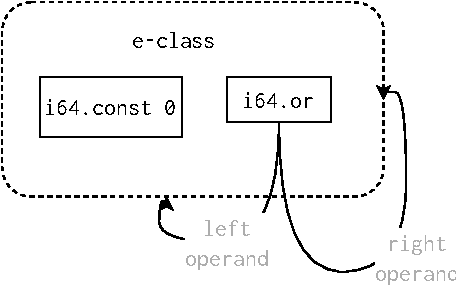
\includegraphics[width=0.7\linewidth]{figures/egraph1.pdf}
    \caption{e-graph for idempotent bitwise-or rewriting rule. Solid lines represent operand-operator relations, and dashed lines represent equivalent class inclusion. }
  \label{e-graph}
\end{figure}

% How to construct
For example, let us consider one program with a single instruction that returns an integer constant, \texttt{i64.const 0}. Let us also assume a single rewriting rule, \texttt{(x,\ x\ i64.or\ x, x instanceof i64)}. 
In this example, the program's control flow graph contains just one node, representing the unique instruction.
The rewriting rule represents the equivalence for performing an \texttt{or} operation with two equal operands.
\autoref{e-graph} displays the final e-graph data structure constructed out of this single program and rewriting rule. 
We start by adding the unique program instruction \texttt{i64.const 0} as an en e-node (depicted by the leftmost solid rectangle node in the figure). 
Next, we generate e-nodes from the rewriting rule (the rightmost solid rectangle) by introducing a new e-node, \texttt{i64.or}, and creating edges to the \texttt{x} e-node.
Following this, we establish equivalence. 
The rewriting rule combines the two e-nodes into a single e-class (indicated by the dashed rectangle node in the figure). 
As a result, we update the edges to point to the \texttt{x} symbol e-class.

%\todo{explain what "equality saturation" means in this context. do we use equality saturation for diversification? I'm not sure}
%Since there are no more rewriting rules to apply, we reach equality saturation, signifying that the graph can no longer change. Therefore, we have successfully constructed the e-graph.

\paragraph{e-graph Traversal Algorithm}
\label{alg}
% General use of case
While e-graphs possess numerous significant properties, we focus on what we believe is the most crucial for the purpose of diversification. We articulate this key attribute as an invariant in the text that follows.

\begin{tcolorbox}[boxrule=1pt,arc=.3em,boxsep=-1.3mm]
Any path traversal through the e-graph results in a semantically equivalent expression
\end{tcolorbox}

%\todo{which invariant? why does it matter?}
The invariant is exemplified in \autoref{e-graph}, where an infinite concatenation of "or" operations can be constructed. 
In this work, we take advantage of this invariant to generate mutated variants of an original program. 
The e-graph can be traversed randomly, selecting an e-node within each e-class that we visit, producing a random-but-equivalent expression. 
%We can extract an infinite number of semantically equivalent expressions from the e-graph, as shown in previous research \cite{10.1145/3571207, 10.1145/3434304}.

%It selects a random instruction within the binary functions and applies one or more of the 125 rewrite rules.
%Finally, it re-encodes the WebAssembly module with the new, rewritten expression to produce a binary variant. 


% - SMT and egraphs are complete different things. Therefore, we need to evaluate the soundness of the egraphs generated programs modulo Input => CROW
 
% - wasm-mutate only applies egraphs if the CFG of the peephole is complete/deterministic.


\algnewcommand\algorithmicforeach{\textbf{for each}}
\algdef{S}[FOR]{ForEach}[1]{\algorithmicforeach\ #1\ \algorithmicdo}
\begin{algorithm}
    \footnotesize
	\begin{algorithmic}[1]
	%	\Procedure{MyProcedure}{}
        \Procedure{traverse}{$egraph$, $eclass$, $depth$}
        % Input:
        %\Comment{Input: e-graph, max-depth}
        % Output:
        %\Comment{Output:y}
        \If{depth = 0}
          \State  \Return \textbf{smallest\_tree\_from}(egraph,\ eclass)
        \Else
            \State $nodes \gets egraph[eclass]$
            \State $node \gets random\_choice(nodes)$
            \State $expr \gets (node, operands=[])$
            \ForEach {$child \in node.children $}
                \State $subexpr \gets \textbf{TRAVERSE}(egraph,\ child,\ depth - 1)$
                \State $expr.operands \gets expr.operands \cup\ \{subexpr\}$
            \EndFor
            \State \Return $expr$
        \EndIf
        \EndProcedure
	\end{algorithmic} 
	\caption{e-graph traversal algorithm.} 
	\label{peephole:mutator}
\end{algorithm}

%\todo{can we make a strong claim here? does everybody maximize simplification with equality saturation? are we the first to do random path in e-grahs?}
We propose an algorithm to randomly traverse an e-graph and generate  semantically equivalent program variants.
The e-graph traversal is summarized in Algorithm \autoref{peephole:mutator}. 
To the best of our knowledge, \tool, is the first practical implementation of the random e-graph traversal algorithm.
It receives an e-graph, an e-class node (initially the root's e-class), and the maximum depth of expression to extract. The depth parameter ensures that the algorithm is not stuck in an infinite recursion. We select a random e-node from the e-class (lines 5 and 6), and the process recursively continues with the children of the selected e-node (line 8) with a decreasing depth. As soon as the depth becomes zero, the algorithm returns the smallest expression out of the current e-class (line 3). The subexpressions are composed together (line 10) for each child, and then the entire expression is returned (line 11). 

\paragraph{Example of a random e-graph traversal}
Let's demonstrate how the proposed traversal algorithm can generate program variants with an example. 
We will illustrate Algorithm \ref{peephole:mutator} using a maximum depth of 1. 
\autoref{example:peeporig} presents a hypothetical original Wasm binary to mutate. 
In this example, the developer has established two rewriting rules: \texttt{(x, x i32.or x, x instanceof i32)} and \texttt{(x, x i32.add 0, x instanceof i32)}. The first rewriting rule represents the equivalence of performing an \texttt{or} operation with two equal operands, while the second rule signifies the equivalence of adding 0 to any numeric value.
By employing the code and the rewriting rules, we can construct the e-graph depicted in \autoref{e-graph3}. The figure demonstrates the operator-operand relationship using arrows between the corresponding nodes.



\lstdefinestyle{watcode}{
  numbers=none,
  stepnumber=1,
  numbersep=10pt,
  tabsize=4,
  showspaces=false,
  breaklines=true, 
  showstringspaces=false,
    moredelim=**[is][{\btHL[fill=weborange!40]}]{`}{`},
    moredelim=**[is][{\btHL[fill=celadon!40]}]{!}{!}
}


   \begin{minipage}[b]{\linewidth}
    \lstset{
        language=WAT,
                        style=watcode,
        basicstyle=\footnotesize\ttfamily,
                        columns=fullflexible,
                        breaklines=true}
        
        \begin{lstlisting}[label=example:peeporig,caption={Wasm function.},frame=b, captionpos=b]{Name}
(module
    (type (;0;) (func (param i32 f32) (result i64)))
    (func (;0;) (type 0) (param i32 f32) (result i64)
        i64.const 1)
)
        \end{lstlisting}
\end{minipage}


\begin{minipage}[b]{\linewidth}
    \lstset{
        language=WAT,
                        style=watcode,
        basicstyle=\footnotesize\ttfamily,
                        columns=fullflexible,
                        breaklines=true}
        
        \begin{lstlisting}[label=example:peepapplied,caption={Random peephole mutation using egraph traversal for \autoref{example:peeporig} over e-graph \autoref{e-graph3}. The textual format is folded for better understanding.},frame=b, captionpos=b]{Name}
(module
    (type (;0;) (func (param i32 f32) (result i64)))
    (func (;0;) (type 0) (param i32 f32) (result i64)
        !(i64.or (!
            !(i64.add (!
                !i64.const 0!
                !i64.const 1!
            !))!
            !i64.const 1!
        !))!
    )
        \end{lstlisting}
\end{minipage}



\begin{figure}
    \centering
    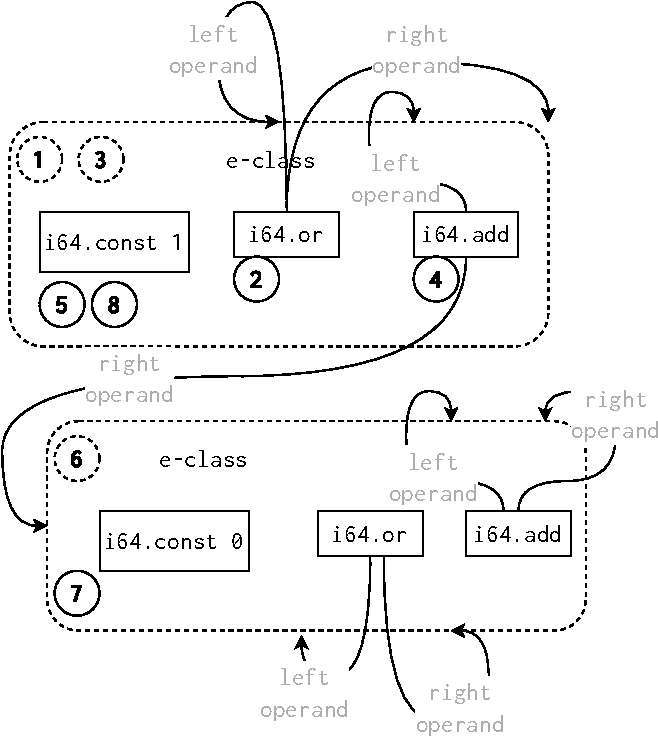
\includegraphics[width=0.9\linewidth]{figures/egraph3.pdf}
    \caption{e-graph built starting in the first instruction of \autoref{example:peeporig}. }
  \label{e-graph3}
\end{figure}


In \autoref{e-graph3}, we annotate the various steps of Algorithm \ref{peephole:mutator} 
for the scenario  described above. Algorithm \ref{peephole:mutator} begins at the e-class containing the single instruction \texttt{i64.const 1} from \autoref{example:peeporig}. 
It then selects an equivalent node in the e-class (2), in this case, the \texttt{i64.or} node, resulting in:
{\texttt{expr = i64.or l r}}.
The traversal proceeds with the left operand of the selected node (3), choosing the \texttt{i64.add} node within the e-class: 
{\texttt{expr = i64.or (i64.add l r)} \texttt{r}}.
The left operand of the \texttt{i64.add} node is the original node (5): 
{\texttt{expr = i64.or (i64.add i64.const 1 r)} \texttt{r}}.
The right operand of the \texttt{i64.add} node belongs to another e-class, where the node \texttt{i64.const 0} is selected (6)(7):
{\texttt{expr = i64.or (i64.add i64.const 1 i64.const 0)} \texttt{r}}.
In the final step (8), the right operand of the \texttt{i64.or} is selected, corresponding to the initial instruction e-node, returning:
{\texttt{expr = i64.or (i64.add i64.const 1 i64.const 0)\ i64.const 1}}
The traversal result applied to the original Wasm code can observed in \autoref{example:peepapplied}. 



\subsection{Implementation}

\tool is implemented in Rust, comprising approximately 10767 lines of Rust code. 
We leverage the capabilities of the wasm-tools project of the bytecodealliance for parsing and transforming WebAssembly binary code. 
Specifically, we utilize the wasmparser and wasm-encoder modules for parsing and encoding Wasm binaries, respectively.
The combination of wasmparser and wasm-encoder enables \tool to rewrite Wasm binaries. 
All operations are done lazily: only the necessary sections of the binary are parsed and rewritten during the transformation of the input Wasm by \tool.
The implementation of \tool can be found at \url{https://github.com/bytecodealliance/wasm-tools}.

%\todo{J: Should we talk about determinism in the transformations?}



%Although the construction of the e-graph itself can be expensive, we can reuse the e-graph many times after construction, amortizing the construction costs. 
%We can also speed up construction by limiting the number of rewrites applied to the e-graph. 


%\textbf{Add global}
%\todo{Move this to special operators in the peephole mutator}
%
\lstdefinestyle{watcode}{
  numbers=none,
  stepnumber=1,
  numbersep=10pt,
  tabsize=4,
  showspaces=false,
  breaklines=true, 
  showstringspaces=false,
    moredelim=**[is][{\btHL[fill=black!10]}]{`}{`},
    moredelim=**[is][{\btHL[fill=celadon!40]}]{!}{!}
}

{\captionsetup{width=0.45\linewidth}
\noindent\begin{minipage}[b]{0.45\linewidth}
    \lstset{
        language=WAT,
        style=watcode,
        basicstyle=\footnotesize\ttfamily,
        columns=fullflexible,
        breaklines=true}
        \begin{lstlisting}[label=example:block1,caption={Add global.},frame=b, captionpos=b]{Name}
...
!+ !
...
        \end{lstlisting}
        %\vspace{0.2cm}
   \end{minipage}\hfill%
\noindent\begin{minipage}[b]{0.45\linewidth}
    \lstset{
        language=WAT,
                        style=watcode,
        basicstyle=\footnotesize\ttfamily,
                        columns=fullflexible,
                        breaklines=true}
        
        \begin{lstlisting}[label=example:block2,caption={Remove global.},frame=b, captionpos=b]{Name}
...
`- `
...   
        \end{lstlisting}
\end{minipage}
}


%\subsection{Properties}

%- Ergodicity (validates malware evasion paper)

%- Faster (compare to other rewriting tools, CROW)

%- Taxonomy, easy to measure and control the rewriting space. Define properties and metrics, e.g. size of the rewriting.

\section {Evaluation}

\todo{Introduce the section}

\todo{NUC specification here}

% \subsection{Research Questions}

\newcommand\rqstatic{To what extent are the program variants generated by \tool statically different?\xspace}

\newcommand\rqdynamic{ To what extent are the program variants generated by \tool dynamically different?\xspace}

\newcommand\rqdefensive{To what extent does \tool prevent Spectre side-channel attacks on \Wasm programs?\xspace}


\newcommand\rqperformance{To what extent does \tool affects \Wasm variants performance?\xspace}

\newcommand\rqofensive{To what extent are the program variants generated by \tool harmful?\xspace}


\newcommand\rqtesting{To what extent can \tool be used to perform differential testing of \Wasm tools?\xspace}

\newcommand{\nProgramsRosetta}{303\xspace}


\newcommand{\DTWStatic}{\ensuremath{\mathit{dt\_static}\xspace}}
\newcommand{\DTWDynamic}{\ensuremath{\mathit{dt\_dy}\xspace}}

\begin{enumerate}[label=RQ\arabic*:, ref=RQ\arabic*]
    % From CROW %%%%%%%%%%%%%%%%%%%%%%%%%%%%%%%%%%%%%%%%%%%%%%%%%%%%%%%%%%%%%%%%%%%
     \item \label{rq:static} \textbf{\rqstatic}
        We  check whether the \wasm binary variants produced by \tool are different from the original \wasm binary. %Then, we assess whether the generation of x86 machine code performed by  wasmtime engine preserves \tool's transformations.
    
    \item \label{rq:dynamic}\textbf{\rqdynamic} 
        It is known that not all diversified programs produce distinguishable executions \cite{crane2015thwarting}, sometimes it is impossible to observe different behaviors between variants. 
        We check for the presence of different behaviors by collecting the execution traces out of wasmtime, characterizing the behavior of a \wasm program by its memory and instruction traces.
    %%%%%%%%%%%%%%%%%%%%%%%%%%%%%%%%%%%%%%%%%%%%%%%%%%%%%%%%%%%%%%%%%%%%%%%%%%%%%%%
        
    \item \label{rq:defensive}\textbf{\rqdefensive} 
     \label{rq:performance} Diversification has been proved to prevent security issues. We asses the impact of \tool in preventing Spectre Proof of Concepts designed for \Wasm.

    \item \label{rq:testing}\textbf{\rqtesting} 
    
    %\item \label{rq:ofensive}\textbf{\rqofensive} 
    
\end{enumerate}

\subsection{Corpus}
\label{sec:corpus}


\begin{table}
\renewcommand\arraystretch{1.1}
\begin{adjustbox}{width=\linewidth,totalheight=\textheight, keepaspectratio}
{
\color{blue}
    \begin{tabular}{p{1.5cm} | l | l | r | r | p{2cm}  }
        \hline
        Source & Program & RQ & \#F & \# Ins. & Attack  \\
        \hline \hline
        CROW \cite{arteaga2020crow} & 303 & \ref{rq:static}, \ref{rq:dynamic} & 7-103 & 170-36,023 & N/A  \\
        \hline

        wasmbench \cite{hilbig2021empirical} & 134 & \ref{rq:performance} & 1-8,375 & 11-1,162,469 & N/A \\
        
        \hline

        Swivel \cite{Swivel} & btb\_breakout & \ref{rq:defensive} & 16 & 743 & Spectre branch target buffer (btb)  \\
        \hline
        Swivel \cite{Swivel}  & btb\_leakage & \ref{rq:defensive} & 16 & 297 & Spectre branch target buffer(btb)  \\
        \hline
        Safeside \cite{Swivel, safeside}  & ret2spec & \ref{rq:defensive} & 2,977 & 378,894 & Spectre Return Stack Buffer (rsb)  \\
        \hline
        Safeside  \cite{Swivel, safeside} & pht & \ref{rq:defensive} & 2,978 & 379,058 & Spectre Pattern History Table (pht)  \\

        

%\end{adjustbox}
    \end{tabular}
}
\end{adjustbox}
    
    \caption{The dataset we use to evaluate \tool. Each row in the table corresponds to programs, with the columns providing: where the program is sourced from, the number of programs, research question addressed, function count, the total number of instructions found in the original \wasm program and the type of attack that the original program was subjected to.}
    \label{tab:corpus}
\end{table}


We answer our research questions with a corpus of 303 + 4 original programs.
These programs are summarized in \autoref{tab:corpus}.
Each row in the table corresponds to programs, with the columns providing the following information: Source of the Program wich identifies where the program was sourced from, Program Count or Name which specifies the number of programs, if multiple programs are from the same source, or the name of the program if the source contains only one, Research Question Addressed, Function Count which provides the total number of functions present in each original \wasm program. Instruction Count which indicates the total number of instructions found in the original \wasm programs, Attack Performed which references the type of attack that the original program was subjected to and Building Process which describes the process employed to convert the source code into the corresponding \wasm programs.

We answer \ref{rq:static} and \ref{rq:dynamic} with the same corpus of programs proposed by Cabrera \etal \cite{arteaga2020crow}, as it is shown in the first row of \autoref{tab:corpus}.
The corpus contains \nProgramsRosetta from Rosetta code, curated in early 2020.
The corpus contains programs in a range of tasks, from simple ones, such as adding two numbers, to complex algorithms like a compiler lexer. 
The number of functions for each program ranges from 7 to 103 and, the number of total instructions ranges from 170 to 36023.
All programs in corpus: 1) do not require input from user, \ie invoking functions like \texttt{scanf}, 2) terminate, 3) are deterministic, \ie given the same input, provide the same output and 4) generates valid \wasm programs when using \texttt{wasi-clang}.

We answer \ref{rq:defensive} with four \Wasm programs and three Spectre attack scenarios, as presented in Swivel \cite{Swivel}. 
These programs are summarized in the final four rows of our corpus table.
The first two programs, manually crafted for simplicity, each contain 16 functions, with instruction counts of 743 and 297, respectively. These binaries are specifically designed to facilitate the execution of the Spectre branch target attack.
The third and fourth programs, documented in rows four and five, correspond to attacks ported from the Safeside project \cite{safeside}. 
Unlike the first two, these binaries are significantly larger, each containing nearly 3000 functions and more than 300000 instructions. 
They are utilized for conducting the Spectre Return Stack (RSB) and Spectre Pattern History (PHT) attacks.
Notice the difference in the number of functions and instructions between the first pair of Swivel binaries and the latter pair. 
This disparity can be attributed to the varying compilation processes applied to these \Wasm binaries. 
The first two were manually tailored to streamline the attack processes, whereas the other two programs were directly compiled from Safeside.
The three attack scenarios are described in details in \autoref{protocol:rq3}.

%% FROM CROW RQ1
\subsection{Protocol for RQ1}


With \ref{rq:static},
we assess the ability of \tool to generate \Wasm binaries that are different from the original program.
For this, we compute the number of unique variants generated by \tool.
To determine if a \wasm variant is unique we calculate the sha256 hash of each variant bytestream.
We run \tool on the CROW's corpus, for a total of \nProgramsRosetta{} original C programs. 
We configure \tool to run with a diversification timeout of 6 hours per program. 

Since \wasm binaries are further transformed into machine code before they execute, we also check that this additional transformation preserves the difference introduces by \tool in the \wasm binary. 
We use the wasmtime and V8 TurboFan ahead-of-time compilers, with all their possible optimizations, to generate the x86 binaries for each \wasm program and its variants. 
Then, we calculate the number of unique variants machine code representation for both compilers.

By also comparing machine codes we consider the following property as diversification preservation: \\
Given two \wasm variants from the same original program $P_{Wasm}$ and $P_{Wasm}'$, where $P_{x86}$ and $P_{x86}'$ are two respective machine codes generated by a JIT compiler:
if $hash(P_{Wasm})$ $\neq$ $hash(P_{Wasm}')$ and $hash(P_{x86}$) $\neq$ $hash(P_{x86}')$, this means that  both programs are still different when compiled to machine code, and we conclude that the \wasm compiler does not remove the transformations made by \tool.  Notice that, this property only makes sense between variants of the same program (including the original).




%% FROM CROW RQ2
\subsection{Protocol for RQ2}

For \ref{rq:dynamic}, we compare  the executions of a program and its variants for a given input. 
We execute the program using a wasmtime embeded host.
In this experiment, we characterize the  execution of a \wasm binary according to its traces.


For each execution of a \wasm program, we collect the instructions and memory traces with IntelPIN. 
To only collect the traces of the Wasm execution with a wasmtime engine, we pause and unpause wheter the execution goes out and in of the Wasm code respectively.
We perform such filtering with the builtin hooks of wasmtime.
Besides, we disable ASLR in the machine where the variants are executed.

For each program we collect two types of traces: executed machine code instructions and memory operations.
An example for such kind of traces can be observed in \todo{listing}.
Collected traces are ordered with respect to the timestamp of the events. 
Once we execute the original program and its variants we calculate the Shannon entropy \cite{shannon} for all collected traces.
The Shannon entropy is defined as follows:

\todo{Double check the metric}

\begin{metric}{Normalized Shannon entropy: $E(e)$}\label{metric:entropy}
    Let $p$ be an original \wasm binary, $C(p)$ be the union  of all traces for all variants of program $p$.
    The normalized Shannon Entropy for the program  $p$ variants over the collected traces is defined as: \\
    {
    \scriptsize
        $$
            E(p)=-\Sigma \frac{p_x*log(p_x)}{log(|C(p)|)}
        $$
    
    }
    Where $p_x$ is the discrete probability of the occurrence of the symbol $x$ over $C(p)$.


    
\end{metric}



\subsection{Protocol for RQ3}
\label{protocol:rq3}

\newcommand{\poct}{\emph{Cache timing POC}\xspace}
\newcommand{\pocd}{\emph{Differential computing POC}\xspace}
\newcommand{\pocp}{\emph{Port contention POC}\xspace}

To answer \ref{rq:defensive}, we apply \tool to the same security Proof of Concepts(POC) 
as the ones used by Narayan et al. to evaluated Swivel's ability at protecting \wasm programs \cite{Swivel}. 
The four cache timing side-channel attacks are presented in detail in \autoref{sec:corpus}. 
We evaluate to what extent \tool can prevent such attacks.
In the following text, we describe the POCs used to answer \ref{rq:defensive}.

%\todo{move the description of the four binaries in  \autoref{sec:corpus} and here add a short description of the intuition why \tool could be useful to prevent the attacks}

% Describing the Speculative execution  POC
Narayan and colleagues successfully navigated around the control flow integrity safeguards outlined in \cite{Swivel} for \Wasm, using speculative code execution as detailed in \cite{Spectre}. 
Thus, we use the same three Spectre attacks evaluated in Swivel.
Which specific binary and its corresponding attack can be appreciated in \autoref{tab:corpus}.
First, Spectre Branch Target Buffer (btb) attack. 
This attack exploits the branch target buffer by predicting the target of an indirect jump, thereby rerouting speculative control flow to an arbitrary target, similar to a ROP-style attack \cite{?}.
Second, Spectre Pattern History Table (pht).
It takes advantage of the pattern history table to anticipate the direction of a conditional branch during the ongoing evaluation of a condition. 
Third, Spectre Return Stack Buffer (ret2spec) attack. 
This attack exploits the return stack buffer that stores the locations of recently executed call instructions to predict the target of \texttt{ret} instructions. 
The attack methodology hinges on the extraction of memory bytes from the host engine and from another hosted \wasm binary.

%\todo{TBD: in the end, I do not think we need this, we are not comparing their approach.}
%Swivel is designed to thwart attacks \cite{Swivel} that rely on three specific low-level instructions supplied by any standard libc implementation: the rdtsc instruction for measuring execution time, the clflush instruction for evicting a particular cache line, and the mfence instruction which allows pending memory operations to complete. 
%These instructions are not commonly accessible to Wasm through WASI implementations.
%Following the assumptions of the initial attack, we have made these instructions available within an embedded wasmtime host implementation. 
%This adaptation simplifies the POC cases.

For each of the four \wasm binaries introduced in \autoref{sec:corpus}, we generated a maximum of 1000 random transformations utilizing 100 distinct seeds. 
This resulted in a total of 100,000 variants for each original \wasm binary.
We then assessed the success rate of attacks across these variants by measuring the bandwidth of the exfiltrated data, that is: the rate of correctly leaked bytes per unit of time. 
To do so, we execute each variant the same setup of Swivel without mitigations.
The bandwidth metric, proposed by Google's Safeside project \cite{safeside}, serves to quantify the effectiveness of countermeasures.
To determine the bandwidth, we executed each variant and examined the exfiltrated data, represented as a sequence of bytes. 
We counted the correctly exfiltrated bytes and divided them by the variant program's execution time. 
It's important to note that this metric captures not only the binary determination of whether the attacks are successful or not, but also the degree to which the data exfiltration is hindered.
For instance, a variant that continues to exfiltrate secret data but does so over an impractical duration would be deemed as having been hardened. 
This approach recognizes that reducing the efficiency of an attack can be nearly as valuable as stopping it.
In the following definition we state the bandwidth metric:

\begin{metric}{Bandwidth:}\label{metric:ber}
Given data $D=\{b_0, b1, ..., b_C\}$ being exfiltrated in time $T$ and $K = {k_1, k_2, ..., k_N}$ the collection of correct data bytes, the bandwidth metric is defined as:
$$
    \frac{|b_i\text{ such that } b_i \in K|}{T}
$$
\end{metric}






%T%o answer \ref{rq:defensive} we compute \autoref{metric:ber} for each original POC program and its variants generated with \tool.

% Describing the port contention  POC
 

%\subsection{Protocol for RQ4}


%\subsection{Traces}




\section{Experimental Results}

\subsection{\rqstatic}
\label{rq:static:results}

\begin{figure*}
    \centering
    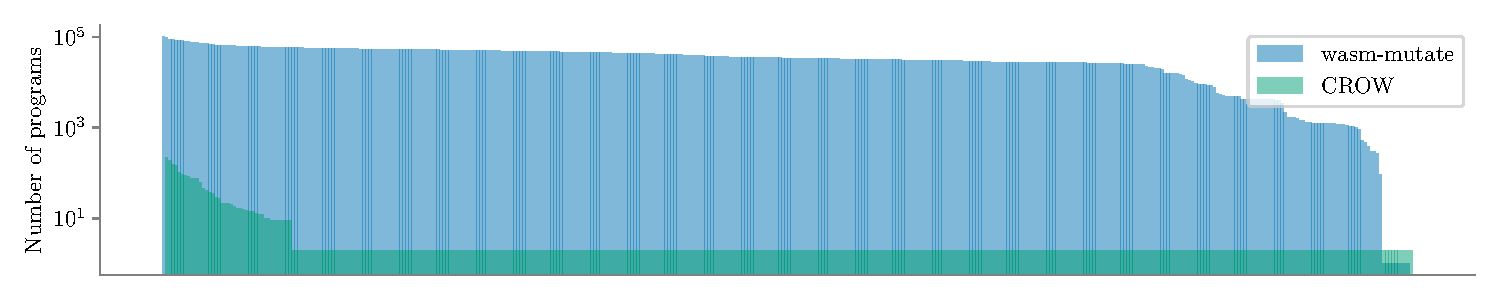
\includegraphics[width=0.9\linewidth]{plots/rq1/count.pdf}
    \caption{TODO.}
  \label{programs_count}
\end{figure*}

\todo{\tool outperform CROW}

\todo{In machine code, the custom section makes no sense. Thus, we might have some pairs that are zero distance in machine code rep.}


\todo{Add discussion on preservation. Take a look to the thesis of Håkon, there are some insights there.}

\todo{Check binary sizes. wasm-mutate optimizes as well. The full spectrum of transformations. }

\todo{Usage as a test case reducer.}

\subsection{\rqdynamic}

\todo{Add comparison of dynamic differences}

\todo{Use the same plot as the Lic...one vert bar per program. The height of the bar is the entropy of the traces of the whole population. The closer to 1 the better. Divide the entropy by the size of the population, then we could compare between programs.}

\todo{\textbf{\rqperformance}}

\subsection{\rqdefensive}



\begin{figure*}
    \centering
    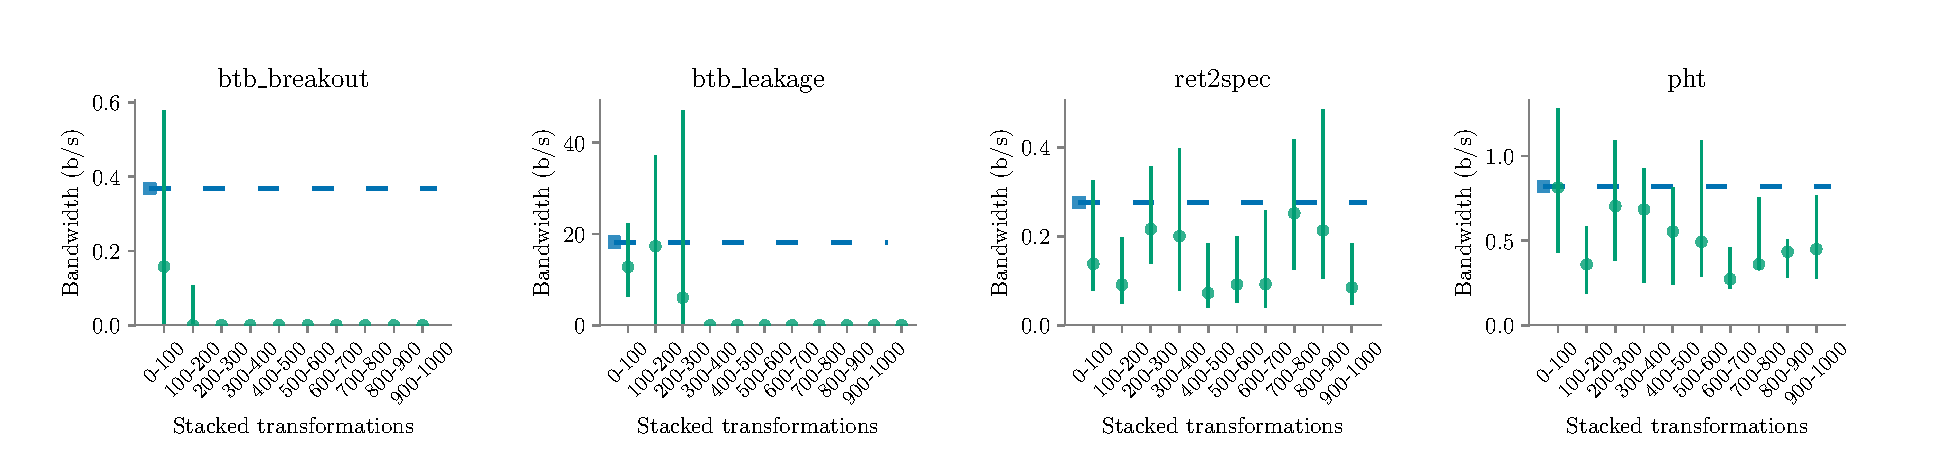
\includegraphics[width=\linewidth]{plots/rq3/results.rq3.pdf}
    \caption{Visual representation of \tool's impact on Swivel's original programs (btb\_breakout, btb\_leakage, ret2spec, and pht) and their associated attacks, shown in sequence from left to right. The Y-axis denotes exfiltration bandwidth, with the original binary's bandwidth under attack highlighted by a blue marker and dashed line. Variants are clustered in groups of 100 stacked transformations, denoted by green dots (median bandwidth) and lines (interquartile bandwidth range). The X-axis marks represent groups with a stacked transformation range from X (minimum) to X + 100 (maximum), with the first green mark aggregating variants with 0 to 100 stacked transformations across all seeds. Overall, for all 100000 variants generated out of each original program, 70\% have less data leakage bandwidth.}
  \label{attacks:impact}
\end{figure*}

To answer \ref{rq:defensive}, we execute \tool on four distinct \wasm susceptible to three Spectre attacks, each of the four programs subjected to a sequence of transformations with 100 different seeds. 
We sequentially stack up to 1000 transformations for each seed. 
At each juncture of the stacking process, we assess the resulting impact of the attacks as outlined in \ref{protocol:rq3}. 
The comprehensive analysis encompasses a total of 4$\times$100$\times$1000 binaries, which also includes the original four.

\autoref{attacks:impact} offers a graphical representation of \tool's influence on the Swivel original programs and their attacks. 
Each subplot corresponds to a specific original \wasm and the attack it undergoes: btb\_breakout, btb\_leakage, ret2spec, and pht, sequenced from left to right.
The Y-axis represents the exfiltration bandwidth. 
The bandwidth of the original binary under attack is portrayed by a blue marker and a corresponding loosely dashed horizontal line.
In each subplot, the variants are grouped in clusters, each encompassing 100 stacked transformations. 
These are indicated by green dots and lines. 
The dot signifies the median bandwidth for the cluster, while the line represents the interquartile range of the group's bandwidth.
Each mark on the X-axis corresponds to a cluster with a range of stacked transformations, starting from a minimum of X to a maximum of X + 100. 
For instance, the first green mark is the aggregation of all variants across all seeds with a minimum of 0 and a maximum of 100 stacked transformations.


% General results for all cases
In the cases of btb\_breakout and btb\_leakage, \tool proves effective, crafting variants that leak less information than the original in 78\% and 70\% of the generated variants respectively. 
For these specific binaries, a remarkable drop in exfiltration bandwidth to zero is observed after 200 stacked transformations across all 100 seeds, a trend clearly showed by the plot. 
Consequently, post 200 stacked transformations, \tool is able to produce variants that are entirely impervious to the original attack.
In the scenarios of ret2spec and pht, the tendency for bandwidth reduction is less prominent. 
Despite this, the generated variants still boast lower bandwidth than the original in 76\% and 71\% of cases respectively. 
It's important to note that in these cases, we have yet to identify variants that leak no correct data to the attacker.


For all cases we have appreciated that the exfiltration bandwidth shows an uptick with a smaller number of stacked transformations, as suggested by the green lines approaching the dashed line. 
This highlights that, while overall the transformations enhance security, the initial few may not always contribute positively to this goal.
We have observed several underlying causes for this phenomenon.


First, as highlighted in previous applications of \tool \cite{CABRERAARTEAGA2023103296}, i.e., uncontrolled diversification may prove to be counterproductive if a specific objective, e.g. with a cost function, is not defined at the outset of the diversification process.
Second, \tool implements certain "symmetric" transformations. 
Specifically, vulnerable code segments may be replicated across the variants, making the variant easier to exploit.
Third, while some transformations result in distinct \wasm binaries, their compilation generates identical machine code. 
Transformations that aren't preserved compromise the efficacy of diversification. 
% This is to answer to the RW of Swivel itself, they proposed ot add nop operations. We know that does not work.
For instance, adding random \texttt{nop} operations directly to \wasm does not alter the final machine code as the \texttt{nop} operations are effortlessly eliminated by the lucet stock compiler.
The same phenomenon occurs with transformations to custom sections of \Wasm binaries.


Lastly, for ret2spec and pht, both show a slight trend towards bandwidth reduction, but this doesn't manifest in a short-term timeframe (low count of stacked transformations).
Moreover, as it can be observe, the exfiltration bandwidth is more scattered for these two programs.
Our analysis suggests a link between these trends and the complexity of the binary undergoing diversification. 
Ret2spec and pht, present significantly more complexity than btb\_breakout and btb\_leakage. 
Specifically, the former includes roughly more than 300000 instructions respectively, whereas the latter two contain no more than 800 instructions.
This substantial disparity in instruction numbers can be attributed to the different creation processes for these binaries. 
The last two were manually crafted to simplify the attacks, while the initial two \wasm programs were compiled directly from safeside. 
In the process of manual crafting, unneeded code was inevitably removed.
Given that \tool implements meticulous, fine-grained transformations one at a time, the probability of influencing key attack components, such as the timer, becomes relatively lower for larger binaries, especially when confined to 1000 transformations. 
Furthermore, it's noteworthy that transformed code doesn't always execute, i.e., \tool might generate dead code.
Based on these observations, we suggest that more  stacked transformations are needed to fully remove the attacks related to ret2spec and pht.


% Why is good, for breaking timers and for padding
On the other hand, as it can be observed in the plots of btb\_breakout and btb\_leakage, the exfiltration bandwidth completely declines after an accumulation of 50 stacked transformations. 
We have discerned the specific types of transformations that produce this result.
All the attacks demonstrated rely on a timer component, responsible for gauging the cache access time for memory lines. 
If this component is disturbed, the precision of the attack is undermined. 
This approach has been deliberately implemented in different contexts as a dynamic approach. 
For instance, Firefox randomizes the built-in JavaScript timer in an effort to diminish the likelihood of potential timing attacks \cite{10.1007/978-3-319-70972-7_13}.
\tool inevitably enables this strategy by introducing instructions in-between the time measurement steps within the \wasm variants.
This method proves effective because the time measurement of single or a few instructions is inherently random. 
By introducing more instructions, this randomness is amplified, thereby reducing the timer's accuracy.
% Mention something about performance here
In \autoref{example:timer} and \autoref{example:timer2}, we illustrate the impact of \tool on timing components. \autoref{example:timer} presents the original access time measurement, while \autoref{example:timer2} showcases a variant where \tool intersperses operations within the time measurement.


\lstdefinestyle{watcode}{
  numbers=none,
  stepnumber=1,
  numbersep=10pt,
  tabsize=4,
  showspaces=false,
  breaklines=true, 
  showstringspaces=false,
    moredelim=**[is][{\btHL[fill=weborange!40]}]{`}{`},
    moredelim=**[is][{\btHL[fill=celadon!40]}]{!}{!}
}


   \begin{minipage}[b]{\linewidth}
    \lstset{
        language=WAT,
                        style=watcode,
        basicstyle=\footnotesize\ttfamily,
                        columns=fullflexible,
                        breaklines=true}
        
        \begin{lstlisting}[label=example:timer,caption={Wasm timer used in btb\_breakout program.},frame=b, captionpos=b]{Name}
;; Code from original btb_breakout
...
(call $readTimer)
(set_local $end_time)
... access to mem
(i64.sub (get_local $end_time ) (get_local $start_time))
(set_local $duration)
...

        \end{lstlisting}
\end{minipage}


\begin{minipage}[b]{\linewidth}
    \lstset{
        language=WAT,
                        style=watcode,
        basicstyle=\footnotesize\ttfamily,
                        columns=fullflexible,
                        breaklines=true}
        
        \begin{lstlisting}[label=example:timer2,caption={Variant of btb\_breakout with more instructions added in between time measurement.},frame=b, captionpos=b]{Name}
;; Variant code
...
(call $readTimer)
(set_local $end_time)
!<inserted instructions>!
... access to mem
!<inserted instructions>!
(i64.sub (get_local $end_time ) (get_local $start_time))
(set_local $duration)
...
        \end{lstlisting}
\end{minipage}


%\todo{J: TBD, I was about to add a piece of code here, but the RQ is already too large. TODO }
Additionally, speculative execution has a limit for the number of instructions it can "cache". 
\tool incorporates instructions in such a manner that the vulnerable instruction falls beyond the cacheable instruction limit. 
This process is referred to as "padding".
The padding changes the layout of the binary code in memory and effectively disrupt the attacker's ability to trigger speculative execution in a harmful way.
Even when an attack is executed and the susceptible code is "speculated", the memory access that has been padded is not.
In Figures \autoref{example:padding} and \autoref{example:padding2}, we demonstrate the influence of \tool on padding instructions. Figure \autoref{example:padding} displays the initial code used to train the branch predictor, along with the anticipated speculated code. In contrast, Figure \autoref{example:padding2} highlights a version where \tool incorporates operations within the time measurement.



\lstdefinestyle{watcode}{
  numbers=none,
  stepnumber=1,
  numbersep=10pt,
  tabsize=4,
  showspaces=false,
  breaklines=true, 
  showstringspaces=false,
    moredelim=**[is][{\btHL[fill=weborange!40]}]{`}{`},
    moredelim=**[is][{\btHL[fill=celadon!40]}]{!}{!}
}


   \begin{minipage}[b]{0.9\linewidth}
    \lstset{
        language=WAT,
                        style=watcode,
        basicstyle=\footnotesize\ttfamily,
                        columns=fullflexible,
                        breaklines=true}
        
        \begin{lstlisting}[label=example:padding,caption={Two jump locations in btb\_breakout. The top one trains the branch predictor, the bottom one is the expected jump that exfiltrates the memory access.},frame=b, captionpos=b]{Name}
;; Code from original btb_breakout
...
;; train the code to jump here (index 1)
(i32.load (i32.const 2000))
(i32.store (i32.const 83)) ;; just prevent optimization
...
;; transiently jump here
(i32.load (i32.const 339968)) ;; S(83) is the secret
(i32.store (i32.const 83)) ;; just prevent optimization
        \end{lstlisting}
\end{minipage}


\begin{minipage}[b]{0.9\linewidth}
    \lstset{
        language=WAT,
                        style=watcode,
        basicstyle=\footnotesize\ttfamily,
                        columns=fullflexible,
                        breaklines=true}
        
        \begin{lstlisting}[label=example:padding2,caption={Variant of btb\_breakout with more instructions added indindinctly between jump places.},frame=b, captionpos=b]{Name}
;; Variant code
...
;; train the code to jump here (index 1)
!<inserted instructions>!
(i32.load (i32.const 2000))
!<inserted instructions>!
(i32.store (i32.const 83)) ;; just prevent optimization
...
;; transiently jump here
!<inserted instructions>!
(i32.load (i32.const 339968)) ;; "S"(83) is the secret
!<inserted instructions>!
(i32.store (i32.const 83)) ;; just prevent optimization
...
        \end{lstlisting}
\end{minipage}


% Performance impact


%\todo{It might be possible to run a test-case reducer...would it work?}

\todo{TBD: Someone might say that the performance is affected and that is why we have less bandwidth. The idea is to answer to this in RQ2. On the other hand, I have collected the times as well, we can show the execution time distribution in cluster as well.}

\begin{tcolorbox}[boxrule=1pt,arc=.3em,boxsep=-1.3mm]
  \textbf{Answer to \ref{rq:defensive}}: \tool successfully provides complete protection for two out of four applications sensitive to Spectre attacks after 200 stacked transformations. 
  For the remaining two applications, it increases their resistance against such attacks by lowering the bandwidth of data exfiltration. 
  We have observed that larger programs necessitate more transformations for effectively neutralizing Spectre attacks.
  Overall, near 70\% of purely random generated variants offer less data leakage bandwidth than their original programs.
\end{tcolorbox}

%\todo{The complexity of the program affects the impact. The larger the program, more difficult to target specific locations. Notions of "knobs". Measure some meta of the original binaries. Number of functions, size in bytes, number of instructions. With more instructions, more the chances to hit the incorrect location.}




%\todo{the pht attack works better. It is more resilient. The reason is related to PHT. Pattern history table attach. Elaborate on this.}


%\todo{Add a figure to show how the traces change. Use tracergraph for it...it will be easier.}


%\tool


\subsection{\rqtesting}

\todo{We break binaryen...that is a good takeaway.}


\todo{Variants generated with wasm-mutate break binaryen ! This might be case 3 !} \todo{We can collect the tools for Wasm presented along all these years and break them, highlighting the need for more testing...this will be nice.}


\section{Threats to validity}

\todo{Diversification migh break other properties, e.g., contant time}

\section{Discussion}

\todo{Fuzzing}

\todo{Evasion}

\todo{Whitebox crypto challenges. While the attack is still possible, we harden it by increasing the attack time :) }

\todo{Synthesis of rewriting rules \cite{10026577}}

\section{Related Work}

In the following text we mention relevant works in the areas of software diversification and the analysis and transformation tools for \Wasm.


% Binary code diversification, static 
\emph{Static diversification} refers to the generation, consolidation, and dissemination of distinct, yet functionally equivalent, binary files to end users. 
The seminal work of Cohen \cite{cohen1993operating} proposed the set of code transformations to produce static diversity.
The main goal of these transformations is to bolster the intricacy and applicability of an attack against a sizeable user base~\cite{cohen1993operating}.
Jackson et al.~\cite{jackson2011compiler} posit that the compiler can be a pivotal element in enabling software diversification. They recommend employing multiple semantic-preserving transformations to facilitate large-scale software diversity, in which each user obtains a uniquely diversified variant.
In relation to code-reuse attacks, Homescu et al.\cite{homescu2013profile} suggest the insertion of NOP instructions directly into the LLVM IR to create a variant that boasts a unique code layout for each compilation. Coppens et al.\cite{coppens2013feedback} also contribute to this field, leveraging compiler transformations to diversify software in an iterative manner. Their research is designed to thwart the reverse engineering of security patches by attackers who target vulnerable programs.
\todo{add a few sentences about the novelty of wasm-mutate wrt these previous work}

% Comparison with CROW
%\todo{write a specific paragraph to explain what specific challenges wasm-mutate addresses that CROW could not address and say how it addresses these challenges}
The innovative tool for software diversification, CROW, draws heavily upon prior techniques, as acknowledged by its creators \cite{arteaga2020crow}. Categorized as a superdiversifier \cite{jacob2008superdiversifier}, CROW situates the LLVM compiler at the very heart of its diversification method.
However, the authors of CROW acknowledge several limitations. 
First, although incorporating the diversifier directly into the LLVM compiler is not intrinsically problematic, it does restrict the tool's scope to those \wasm binaries generated via LLVM. 
In other words, any \wasm source code without an LLVM frontend implementation is unable to benefit from CROW's functionalities.
Conversely, \tool presents the same diversification techniques as CROW, but with a more universal \wasm to \wasm solution, making it compiler agnostic. Significantly, \tool integrates these techniques through a generic rule engine intended for software diversification, enhancing its versatility.
Second, unlike CROW, \tool does not utilize a SMT solver to verify the generated variants, it guarantees semantically equivalence by design. 
As a result, \tool is more efficient in generating \wasm variants, as detailed in \autoref{rq:static:results}.
Finally, \tool enhances the capabilities of CROW by incorporating memory-like transformations. 
While CROW and \tool are not necessarily mutually exclusive in their application, it's worth noting that the rewriting rules of \tool must be manually specified. 
This process, however, could potentially be automated using CROW. 
For instance, a comprehensive set of rewriting rules could be collated and mined from it.

% For example, a custom rewriting rule could be  )
The process of diversifying a WebAssembly (\wasm) program can be conceptualized as a three-stage procedure: parsing the program, transforming it, and finally re-encoding it back into \wasm. 
Our review of the literature has revealed several studies that have employed parsing and encoding components for \wasm binaries across various domains. 
This indicates that these works accept a \wasm binary as an input and output a unique \wasm binary. 
These domains span optimization \cite{wasmslim}, control flow \cite{10123627}, and dynamic analysis \cite{wasabi, stievenart2020compositional, 10123627, BRITO2022102745}.
When the transformation stage introduces randomized mutations to the original program, the aforementioned tools could potentially be construed as diversifiers \cite{some paper claming this}.
However, as they have been custom-built for specific tasks, these tools lack the necessary adaptability to function as all-purpose diversifiers. 
Interestingly, the other side of the coin is possible with \tool.
For instance, \tool can serve as both an optimizer and a test case reducer due to the incorporation of an e-graph at the heart of its diversification process \cite{10.1145/1480881.1480915}. 
To the best of our knowledge, the introduction of an e-graph into \tool marks the first endeavor to integrate an e-graph into a \wasm to \wasm analysis tool.



%\todo{and so what is the main conclusion here? that we could not reuse these tools for diversification? that  \tool could be used for some of these tasks? do some tools use e-graphs? is that the main novelty of \tool regarding wasm analysis?}

BREWasm \cite{rewritingtool2023} offers a comprehensive static binary rewriting framework for \Wasm and can be considered to be the most similar to \tool. 
It parses a Wasm binary into objects, rewrites them using fine-grained APIs, integrates these APIs to provide high-level ones, and re-encodes the updated objects back into a valid Wasm binary. 
The effectiveness and efficiency of BREWasm have been demonstrated through various Wasm applications and case studies on code obfuscation, software testing, program repair, and software optimization. 
%\todo{I don't understand the following 2 sentences. What are the main differences between \tool and BREWasm? in their input? in their output? in their purpose? in their technical approach? }
BREWasm implementation follows a completely different technical approach.
In comparison with our tool, the authors pointed out that our tool employs lazy parsing of Wasm. 
Although they perceived this as a limitation, it is eagerly implemented to accelerate the generation of \wasm binaries.
Additionally, our tool leverages the parser and encoder of wasmtime, a standalone compiler and interpreter for Wasm, thereby boosting its reliability and lowering its error-prone nature.
Madvex \cite{madvex}, on the other hand, alters Wasm binaries with the goal of eluding malware detectors according to a generic reward function, which involves applying transformations to the code to improve malware evasion. 
Their approach primarily focuses on modifying the code section of an input Wasm binary. 
\tool has previously been tested and proven successful for such a task \cite{CABRERAARTEAGA2023103296}, demonstrating its capacity to employ a broader range of transformations, not confined solely to the code section.



\subsection{Some other works to be cited along with the paper. Mostly in the Intro}

\emph{Spectre and side-channel defenses}

- paper 2021: Read this, since it is super related, \url{https://www.isecure-journal.com/article_136367_a3948a522c7c59c65b65fa87571fde7b.pdf} \cite{WasmSpectre}


- A dataset of Wasm programs: \cite{nicholson2023wasmizer}

- Papers 2020

- Papers 2019
- \cite{10.1145/3510003.3510070}

Selwasm: A code protection mechanism for webassembly


Babble

- https://arxiv.org/pdf/2212.04596.pdf

Principled Composition of Function Variants for Dynamic
Software Diversity and Program Protection

- https://dl.acm.org/doi/10.1145/3551349.3559553

How Far We’ve Come – A Characterization Study of Standalone WebAssembly Runtimes

- https://ieeexplore.ieee.org/document/9975423

Code obfuscation against symbolic execution attacks

Code artificiality: A metric for the code stealth based on an n-gram model

Semantics-aware obfuscation scheme prediction for binary

Wobfuscator: Obfuscating javascript malware via opportunistic translation to webassembly

Synthesizing Instruction Selection Rewrite Rules from RTL using SMT
"We also synthesize integer rewrite rules from WebAssembly to RISC-V "

Wafl: Binary-only webassembly fuzzing with fast snapshots


\section{Conclusion}



\bibliographystyle{ACM-Reference-Format}
\bibliography{main}


\end{document}
\endinput
%%
%% End of file `sample-sigplan.tex'.


https://dl.acm.org/doi/pdf/10.1145/3547622